\chapter{Software Design}

\section{Version}
\begin{table}[h]
	\centering
	\begin{tabularx}{\textwidth - 2cm}{|l|l| l|X|}
	\hline
	Dato	& Version	& Initialer & Ændring	\\ \hline
	14. november & 1 & KT	& Første udkast af dokumentet efter review. \\ \hline
	15. december & 2 & LS & Små rettelser. Endelig version. \\ \hline
	\end{tabularx}
\end{table}

\section{PC blokken}

\subsection{Action (Kristian T.)}

\begin{figure}[h]
\centering
\includegraphics[scale=1,clip=true, trim=389 282 302 204.7]{Systemarkitektur/diagrammer/PC_KlasseDiagram} %L B R T - HUSKE DET
\caption{Action klassen}
\end{figure}

%setCommand (1)
\begin{table}[h] 
\begin{tabularx}{\textwidth}{p{0.6 cm} l X} %\hline
\multicolumn{3}{l}{\textbf{setCommand}}\\
& Operation: & %Skriv tekst herunder
\texttt{bool setCommand( int commandNo )}
\\ & Parametre: & %Skriv tekst herunder
Modtager nummeret på den kommando der skal eksekveres.

1 = Tænd

2 = Sluk

3 = Dim 5\%

4 = Dim 15\%

\ldots 

12 = Dim 95\%

\\ & Returværdi: & %Skriv tekst herunder
Returnerer \texttt{TRUE}, hvis input var gyldigt og \texttt{FALSE} hvis ikke.
\\ & Beskrivelse: & %Skriv tekst herunder
Set-metode til at vælge hvilken kommando, den givne aktion skal indeholde. Metoden ændrer udelukkende på variablerne \texttt{commandNo}.
\\ \end{tabularx}
\end{table}

%setUnit
\begin{table}[h] 
\begin{tabularx}{\textwidth}{p{0.6 cm} l X} %\hline
\multicolumn{3}{l}{\textbf{setUnit}}\\
& Operation: & %Skriv tekst herunder
\texttt{bool setUnit( int unitNo )} 
\\ & Parametre: & %Skriv tekst herunder
Modtager hvilken enhed aktionen skal manipulere.

1 = Lampe 1

2 = Lampe 2

3 = TV

4 = Radio

Alle andre værdier er ugyldige. 
\\ & Returværdi: & %Skriv tekst herunder
Returnerer \texttt{TRUE}, hvis input var gyldigt og \texttt{FALSE} hvis ikke.
\\ & Beskrivelse: & %Skriv tekst herunder
Set-metode til at vælge hvilken enhed, den givne aktion skal manipulere. Metoden ændrer udelukkende på variablerne \texttt{houseCode} og \texttt{unitCode}. \texttt{houseCode} skal iøvrigt sættes i forhold til den enhed, som vælges. Lampe 1 og Lampe 2 er under huskode 1, TV og Radio er under hhv. 2 og 3.
\\ \end{tabularx}
\end{table}

%setTime
\begin{table}[h] 
\begin{tabularx}{\textwidth}{p{0.6 cm} l X} %\hline
\multicolumn{3}{l}{\textbf{setTime}}\\
& Operation: & %Skriv tekst herunder
\texttt{bool setTime( int time ) }
\\ & Parametre: & %Skriv tekst herunder
Modtager tidspunktet for hvornår en aktion skal udføres i minutter fra kl \texttt{00:00}. Dvs hvis en aktion skal starte kl \texttt{15:30} skal værdien $15 \times 60 + 30 = 930$ indsættes.
\\ & Returværdi: & %Skriv tekst herunder
Returnerer \texttt{TRUE}, hvis input var gyldigt og \texttt{FALSE} hvis ikke.
\\ & Beskrivelse: & %Skriv tekst herunder
Set-metode til at vælge hvilket tidspunkt, den givne aktion skal udføres. Metoden ændrer udelukkende på variablen \texttt{minutes}.
\\ \end{tabularx}
\end{table}

%operator<<
\begin{table}[h] 
\begin{tabularx}{\textwidth}{p{0.6 cm} l X} %\hline
\multicolumn{3}{l}{\textbf{operator{<}{<}}}\\
& Operation: & %Skriv tekst herunder
\texttt{ostream \& operator{<}{<}( ostream \& theStream, Action \& theAction ) }
\\ & Parametre: & %Skriv tekst herunder
Modtager et \texttt{ostream} objekt, som der skal streames til samt en reference til et objekt af klassen \texttt{Action}, som skal udskrives.
\\ & Returværdi: & %Skriv tekst herunder
Returnerer en reference til det \texttt{ostream} objekt, som metoden blev kaldt med (tillader cascading).
\\ & Beskrivelse: & %Skriv tekst herunder
Udskriver en linie med tidspunkt i formattet \texttt{HH:MM}, enhedsnavn og kommando beskrevet i tekstform, afsluttet med et linieskift.
\\ \end{tabularx}
\end{table}

%Explicit constructor
\begin{table}[h] 
\begin{tabularx}{\textwidth}{p{0.6 cm} l X} %\hline
\multicolumn{3}{l}{\textbf{Explicit constructor}}\\
& Operation: & %Skriv tekst herunder
\texttt{Action( int time, int unit,  int commandNo ) }
\\ & Parametre: & %Skriv tekst herunder
Modtager parametre for hhv. tid, enhed og kommandonummer.
\\ & Beskrivelse: & %Skriv tekst herunder
Initierer attributter i objektet, skal sætte attributterne til passende default-værdier, hvis ingen værdier gives.
\\ \end{tabularx}
\end{table}

\begin{table}[h]
\centering
\begin{tabularx}{13 cm}{|l |X|} \hline
Attribut & Beskrivelse \\ \hline
\texttt{int seconds} & Tiden fra kl \texttt{00:00} til tiden for at den pågældende aktion skal udføres i sekunder. \\ \hline
\texttt{int houseCode} & Huskoden for den enhed, som aktionen skal manipulere. \\ \hline
\texttt{int unitCode} & Enhedskoden for den enhed, som aktionen skal manipulere. \\ \hline
\texttt{int commandNo} & Nummeret på den kommando, som skal eksekveres. \\ \hline
\end{tabularx}
\end{table}

\clearpage

\subsection{Pc controller}

\begin{figure}[h]
\centering
\includegraphics[scale=1,clip=true, trim=267 444 473 60]{Systemarkitektur/diagrammer/PC_KlasseDiagram} %L B R T - HUSKE DET
\end{figure}

PC controlleren virker som et main program, og holder styr på følgende:

\begin{itemize}
\item Kodelås
\item Data til UART klassen
\item Led mellem Scenario og UI klassen
\end{itemize}


\subsection{Scenario (Kristian S.)}

\begin{figure}[h]
\centering
\includegraphics[scale=1,clip=true, trim=149 320 541 224]{../Projektdokumentation/Systemarkitektur/diagrammer/PC_KlasseDiagram.pdf} %L B R T - HUSKE DET
\end{figure}

\begin{table}[h]
\begin{tabularx}{\textwidth}{p{0.6 cm} l X} %\hline
\multicolumn{3}{l}{\textbf{Constructor}}\\
& Operation: & 
\texttt{void Scenario()}  
\\ & Parametre: & 
-
\\ & Returværdi: & 
-
\\ & Beskrivelse: & 
constructoren opretter et array med 20 objekter af klassen action i.
\\ \end{tabularx}
\end{table}

\begin{table}[h]
\begin{tabularx}{\textwidth}{p{0.6 cm} l X} %\hline
\multicolumn{3}{l}{\textbf{getAction}}\\
& Operation: & 
\texttt{Action \& getAction(int actionNo)}  
\\ & Parametre: & 
actionNo - ID'et på den action er der skal bruges
\\ & Returværdi: & 
Action \& - Reference til den valgte action.
\\ & Beskrivelse: & 
Methoden finder den valgte Action ud fra parameteren \texttt{actionNo}, og returnere en reference til den action.
\\ \end{tabularx}
\end{table}

\begin{table}[h]
\begin{tabularx}{\textwidth}{p{0.6 cm} l X} %\hline
\multicolumn{3}{l}{\textbf{sortActions}}\\
& Operation: & 
\texttt{Action[] \& sortActions( Action[] )}  
\\ & Parametre: & 
Modtager en pointer til et array af \texttt{Action} objekter.
\\ & Returværdi: & 
Returnerer en reference til det sorterede array af \texttt{Action} objekter.
\\ & Beskrivelse: & 
Sorterer et array af \texttt{Action} objekter efter udførelsestidspunkt. Den der skal udføres først lægges i starten af arrayet. Alt skal være relativt til det nuværende tidspunkt.
\\ \end{tabularx}
\end{table}

%operator<<
\begin{table}[h]
\begin{tabularx}{\textwidth}{p{0.6 cm} l X} %\hline
\multicolumn{3}{l}{\textbf{operator{<}{<}}}\\
& Operation: & 
\texttt{ostream \& operator{<}{<}( ostream \& theStream, Scenario \& theScen )}  
\\ & Parametre: & 
Modtager det \texttt{ostream} objekt, som der skal streames til samt hvilket \texttt{Scenario} objekt, der skal streames.
\\ & Returværdi: & 
Returnerer en reference til det \texttt{ostream} objekt, der modtages som parameter. (tillader cascading).
\\ & Beskrivelse: & 
Skal udskrive ''Aktionsnummer  Tidspunkt  Enhed  Kommando'' som titler med et bestemt mellemrum på én linie og herefter udskrive nummeret på den første aktion, den første aktion på den næste linie. Herefter udskrives nummeret på den anden aktion samt den anden aktion på den næste linie osv. Se evt. Tabel \ref{tbl:kommando} på side \pageref{tbl:kommando} i kravspecifikationen.
\\ \end{tabularx}
\end{table}

\clearpage

\subsection{UART (Kasper)}

\begin{figure}[h]
\centering
\includegraphics[scale=1,clip=true, trim=448 440 225 50]{Systemarkitektur/diagrammer/PC_KlasseDiagram} %L B R T - HUSKE DET
\end{figure}

UART'en laves med udgangspunkt i funktionerne fra et open-source UART projekt. \cite{lib:UART}

\begin{table}[h]
\begin{tabularx}{\textwidth}{p{0.6 cm} l X} %\hline
\multicolumn{3}{l}{\textbf{Connect}}\\
& Operation: & 
\texttt{Void Connect()}
\\ & Parametre: & 
 - 
\\ & Returværdi: & 
-
\\ & Beskrivelse: & 
Connect methoden bruges til at finde en gyldig USB port hvor i der er indsat et RS-232 stik som bruges til seriel kommunikation. methoden løber igennem alle gyldige COM-porte på PC'en indtil en port, med RS-232 stik i, findes.
\\ \end{tabularx}
\end{table}

\begin{table}[h]
\begin{tabularx}{\textwidth}{p{0.6 cm} l X} %\hline
\multicolumn{3}{l}{\textbf{getLockStatus}}\\
& Operation: & 
\texttt{bool getLockStatus( void)}
\\ & Parametre: & 
 - 
\\ & Returværdi: & 
bool: returnere \texttt{true} / \texttt{false} afhængeligt af kodelåsens status.
\\ & Beskrivelse: & 
Sender ASCII værdien for et \texttt{L} over til microcontrolleren for at få kodelåsens status. Funktionen venter på at få et svar tilbage fra microcontrolleren, hvilket er ASCII værdien for et \texttt{U} eller et \texttt{L}.
Hvis UART'en får et \texttt{L} returneres \texttt{True}.
Hvis UART'en får et \texttt{U} returneres \texttt{False}.
\\ \end{tabularx}
\end{table}

\begin{table}[h]
\begin{tabularx}{\textwidth}{p{0.6 cm} l X} %\hline
\multicolumn{3}{l}{\textbf{stopAll}}\\
& Operation: & 
\texttt{void stopAll(void)}
\\ & Parametre: & 
 - 
\\ & Returværdi: & 
-
\\ & Beskrivelse: & 
Funktionen bruges til at slukke for alle enheder tilsluttet systemet. ASCII værdien for et \texttt{S} sendes for til  microcontrolleren. Se evt. Protokol for UART side \pageref{prot_UART}.
\\ \end{tabularx}
\end{table}

\begin{table}[h]
\begin{tabularx}{\textwidth}{p{0.6 cm} l X} %\hline
\multicolumn{3}{l}{\textbf{SendScen}}\\
& Operation: & 
\texttt{void SendScen(Scenario \& Scenario)}
\\ & Parametre: & 
 Scenario \& Scenario: reference til scenariet.
\\ & Returværdi: & 
-
\\ & Beskrivelse: & 
UARTen transmittere data over serial kommunikation. Rækkefølgen på data der bliver sendt er følgende:
Unit (1 char) \- CMD(1char) \- Time (2char).
datarækken bliver sendt 20 gange for at få alle kommandoer i scenariet overført til microcontroller. 		

NOTE: Tiden omreges iforhold til nuværende tid på systemet i computeren.
f.eks. hvis klokken er 15.00 på computeren og første aktion sker kl 16.30 bliver tiden sat som 90.

\\ \end{tabularx}
\end{table}

\clearpage

\subsection{UI (Kasper)}
 
\begin{figure}[h]
\centering
\includegraphics[scale=1,clip=true, trim=38 433 625 50]{../Projektdokumentation/Systemarkitektur/diagrammer/PC_KlasseDiagram} %L B R T - HUSKE DET
\end{figure}

\begin{table}[h]
\begin{tabularx}{\textwidth}{p{0.6 cm} l X} %\hline
\multicolumn{3}{l}{\textbf{drawMainMenu}}\\
& Operation: & 
\texttt{int drawMainMenu( void )} 
\\ & Parametre: & 
 -
\\ & Returværdi: & 
int : Den returnerede integer er hvilken menu der er valgt.
\\ & Beskrivelse: & 
Metoden udskriver en menu over de forskellige undermenuer på skærmen og giver brugeren muligheden for at vælge at gå ind i en af undermenuerne (opret nyt scenarie(1), kør eksisterende scenarie(2), stop scenarie(3)). Der fortages et tjek på det indtastede af brugeren, som skal valideres. validationen tjekker at det indtastede er enten 1,2 eller 3 som er de gyldige menu'er. hvis det indtastede er ugyldigt får brugeren en besked om ugyldigt input og får lov at forsøge igen. Dette sker indtil brugeren indtaster noget gyldigt.
\\
\end{tabularx}
\end{table}

\begin{table}[h]
\begin{tabularx}{\textwidth}{p{0.6 cm} l X} %\hline
\multicolumn{3}{l}{\textbf{drawScenario}}\\
& Operation: & 
\texttt{int drawScenario( Scenario \& currentScen )} 
\\ & Parametre: & 
Scenario \& currentScen : reference til klassen Scenario
\\ & Returværdi: & 
int : Den returnerede værdi er den valgte action i Scenariet
\\ & Beskrivelse: & 
Metoden udskriver en liste over de 20 aktioner der er i scenariet med at bruge ostream operatoeren der er lavet i klassen \texttt{Scenarie}. Brugeren kan derefter vælge hvilken af de 20 aktioner der skal redigeres ved at indtaste nummeret på aktionen. Når brugeren har indtastet noget, valideres dette. Hvis inputtet er den af de gyldige værdier (0-19), returneres ID'et/den gyldige værdi. Hvis inputtet er ugyldigt får brugeren en besked om ugyldigt input og får lov at forsøge igen. Dette sker indtil brugeren indtaster noget gyldigt.
\\
\end{tabularx}
\end{table}

\begin{table}[h]
\begin{tabularx}{\textwidth}{p{0.6 cm} l X} %\hline
\multicolumn{3}{l}{\textbf{drawAskUnits}}\\
& Operation: & 
\texttt{int drawAskUnits( void )} 
\\ & Parametre: & 
 -
\\ & Returværdi: & 
int : Den returnerede integer er hvilken unit der valgt
\\ & Beskrivelse: & 
Metoden udskriver en liste over units. hvor unitsne er: Lampe1, Lampe2, TV og Radio.
brugeren kan derefter vælge hvilke af de 4 units der skal bruges, ved at indtaste nummeret på unit'en.
Når brugeren har indtastet noget, valideres dette. Hvis inputtet er en af de gyldige værdier (1-4) returneres unit ID'en/den gyldige værdi. Hvis inputtet er ugyldigt får brugeren en besked om ugyldigt input og får lov at forsøge igen. Dette sker indtil brugeren indtaster noget gyldigt.
\\
\end{tabularx}
\end{table}

\begin{table}[h]
\begin{tabularx}{\textwidth}{p{0.6 cm} l X} %\hline
\multicolumn{3}{l}{\textbf{drawAskCommando}}\\
& Operation: & 
\texttt{int drawAskCommand( void )} 
\\ & Parametre: & 
 -
\\ & Returværdi: & 
int : Den returnerede integer er hvilken kommando
\\ & Beskrivelse: & 
Metoden udskriver en liste over kommandoer. Brugeren kan derefter vælge hvilken kommando der skal bruges, og ID'en på denne kommando returneres. 
\\
\end{tabularx}
\end{table}

\begin{table}[h]
\begin{tabularx}{\textwidth}{p{0.6 cm} l X} %\hline
\multicolumn{3}{l}{\textbf{drawAskTime}}\\
& Operation: & 
\texttt{int drawAskTime( void )} 
\\ & Parametre: & 
 -
\\ & Returværdi: & 
int : tiden i minutter indtastet af brugeren siden kl 00.00
\\ & Beskrivelse: & 
Metoden beder brugeren om at indtaste den ønskede time-tal, hvor en ønsket kommando skal udføres. Brugeren kan derefter indtaste det ønskede time-tal. 
Metoden beder nu brugeren om at indtaste det ønskede minut-tal i den ønskede time. Brugeren kan nu indtaste det ønskede minut-tal. Metoden validere nu time- og minut-tallene. hvis time-talet er indenfor det gyldige område (0-23) og minut-talet er indenfor dens gyldige område (0-59), udregnes tiden i minutter siden kl 00.00 og returneres. Hvis enten minut- eller time-tal er udenfor det gyldige område, køres metoden fra starten af, og dette sker indtil den gyldig tid indtastes.
\\
\end{tabularx}
\end{table}

\begin{table}[h]
\begin{tabularx}{\textwidth}{p{0.6 cm} l X} %\hline
\multicolumn{3}{l}{\textbf{drawScenList}}\\
& Operation: & 
\texttt{int drawScenList( void )} 
\\ & Parametre: & 
 -
\\ & Returværdi: & 
int : ID'et på det valgte scenarie
\\ & Beskrivelse: &
Brugeren bliver præsenteret for 3 forudstillede scenarier, med beskrivelser af hvad de gør. Brugeren vælger en af de 3 forudinstillet scenarier, ved at indtaste nummeret på det ønskede scenarie. Det indtastede valideres. Hvis det indtastede er indenfor området 1-3, returneres det indtastede, ellers bliver brugeren bedt om at prøve igen, indtil noget gyldigt er indtastet.
\end{tabularx}
\end{table}

\clearpage

\begin{table}[h]
	\begin{tabularx}{\textwidth}{p{0.6 cm} l X} %\hline
	\multicolumn{3}{l}{\textbf{drawStopPromt}}\\
	& Operation: & 
	\texttt{bool drawStopPromt( void )} 
	\\ & Parametre: & 
	 -
	\\ & Returværdi: & 
	bool: returnere \texttt{true} for valgt 'ja' og \texttt{false} for valgt nej
	\\ & Beskrivelse: & 
	Brugeren bliver præsenteret med muligheden om brugeren er sikker på at scenariet skal afsluttes. Hvis brugeren trykker på \texttt{Y / y} tasten returneres dette som et \texttt{true}, altså et 'ja'. hvis alt andet end \texttt{Y / y} trykkes returneres \texttt{false}, svarende til et 'nej'.
\end{tabularx}
\end{table}

\clearpage

\section{Transmitter blokken}

\subsection{Action (Kristian T.)}

\begin{figure}[h]
\centering
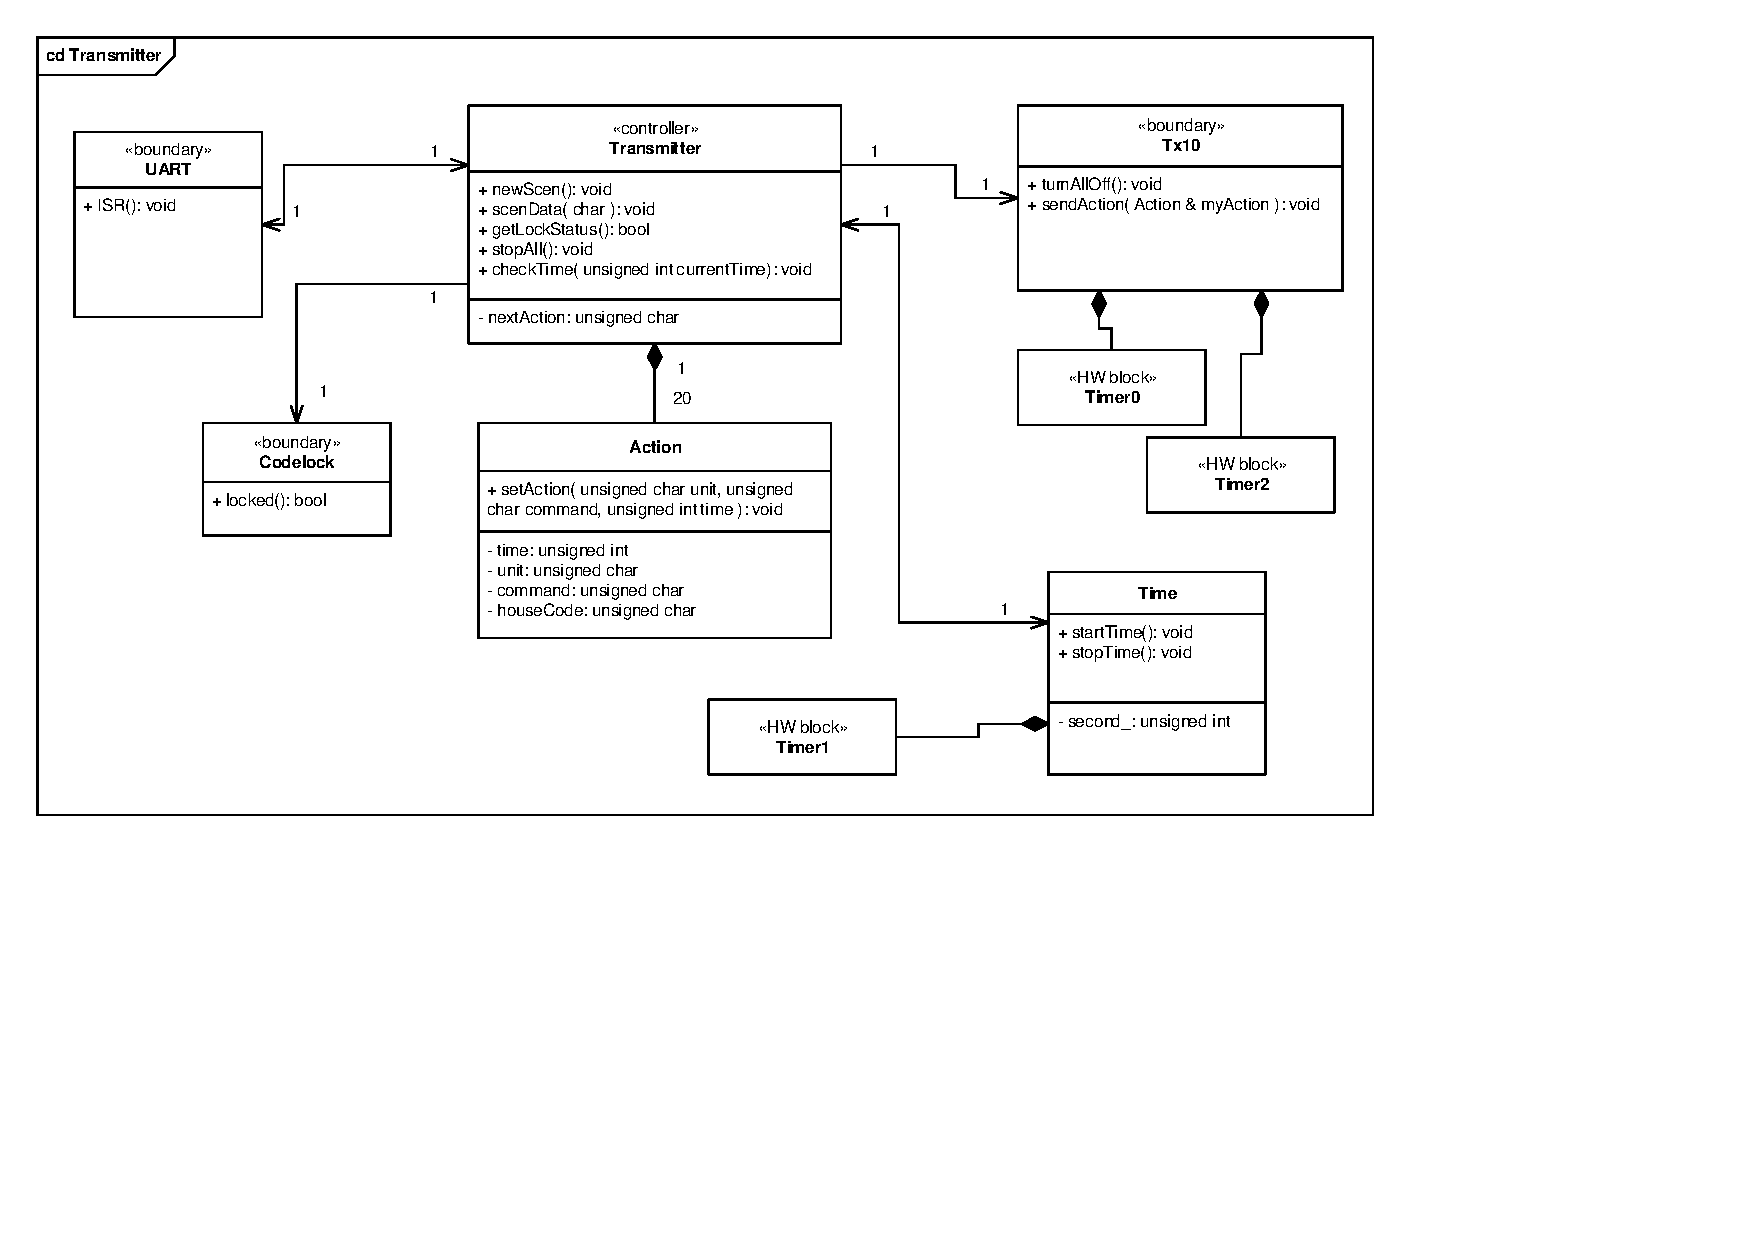
\includegraphics[scale=1,clip=true, trim=210 288 442.4 203]{Systemarkitektur/diagrammer/Transmitter_Klassediagram} %L B R T - HUSKE DET
\end{figure}

%setAction
\begin{table}[h]
\begin{tabularx}{\textwidth}{p{0.6 cm} l X} %\hline
\multicolumn{3}{l}{\textbf{setAction}}\\
& Operation: & %Skriv tekst herunder
\texttt{void setAction( unsigned char unit, unsigned char command, unsigned int time ) }
\\ & Parametre: & %Skriv tekst herunder
Modtager enhed, kommando og tidspunkt relativt til starttidspunktet for aktionen.
\\ & Returværdi: & %Skriv tekst herunder
-
\\ & Beskrivelse: & %Skriv tekst herunder
Metodens formål er primært at gemme informationer i en aktion. Metoden skal selv sætte houseCode baseret på hvilken enhed, den kaldes med. De forskellige houseCode værdier kan ses nedenfor:

Lamper: 1

TV: 2

Radio: 3
\\ \end{tabularx}
\end{table}


%attributter
\begin{table}[h]
\centering
\begin{tabularx}{13 cm}{|l |X|} \hline
Attribut & Beskrivelse \\ \hline

\texttt{unsigned int time} & Gemmer tiden i minutter for den pågældende aktion relativt til det tidspunkt scenariet sættes igang. \\ \hline
\texttt{unsigned char unit} & Gemmer hvilken enhed, aktionen skal gælde for. \\ \hline
\texttt{unsigned char command} & Gemmer hvilken kommando, aktionen skal sende. \\ \hline
\texttt{unsigned char houseCode} & Gemmer huskoden, for den enhed der skal manipuleres. \\ \hline
\end{tabularx}
\end{table}

\clearpage
\subsection{Codelock (David)}

\begin{figure}[h]
\centering
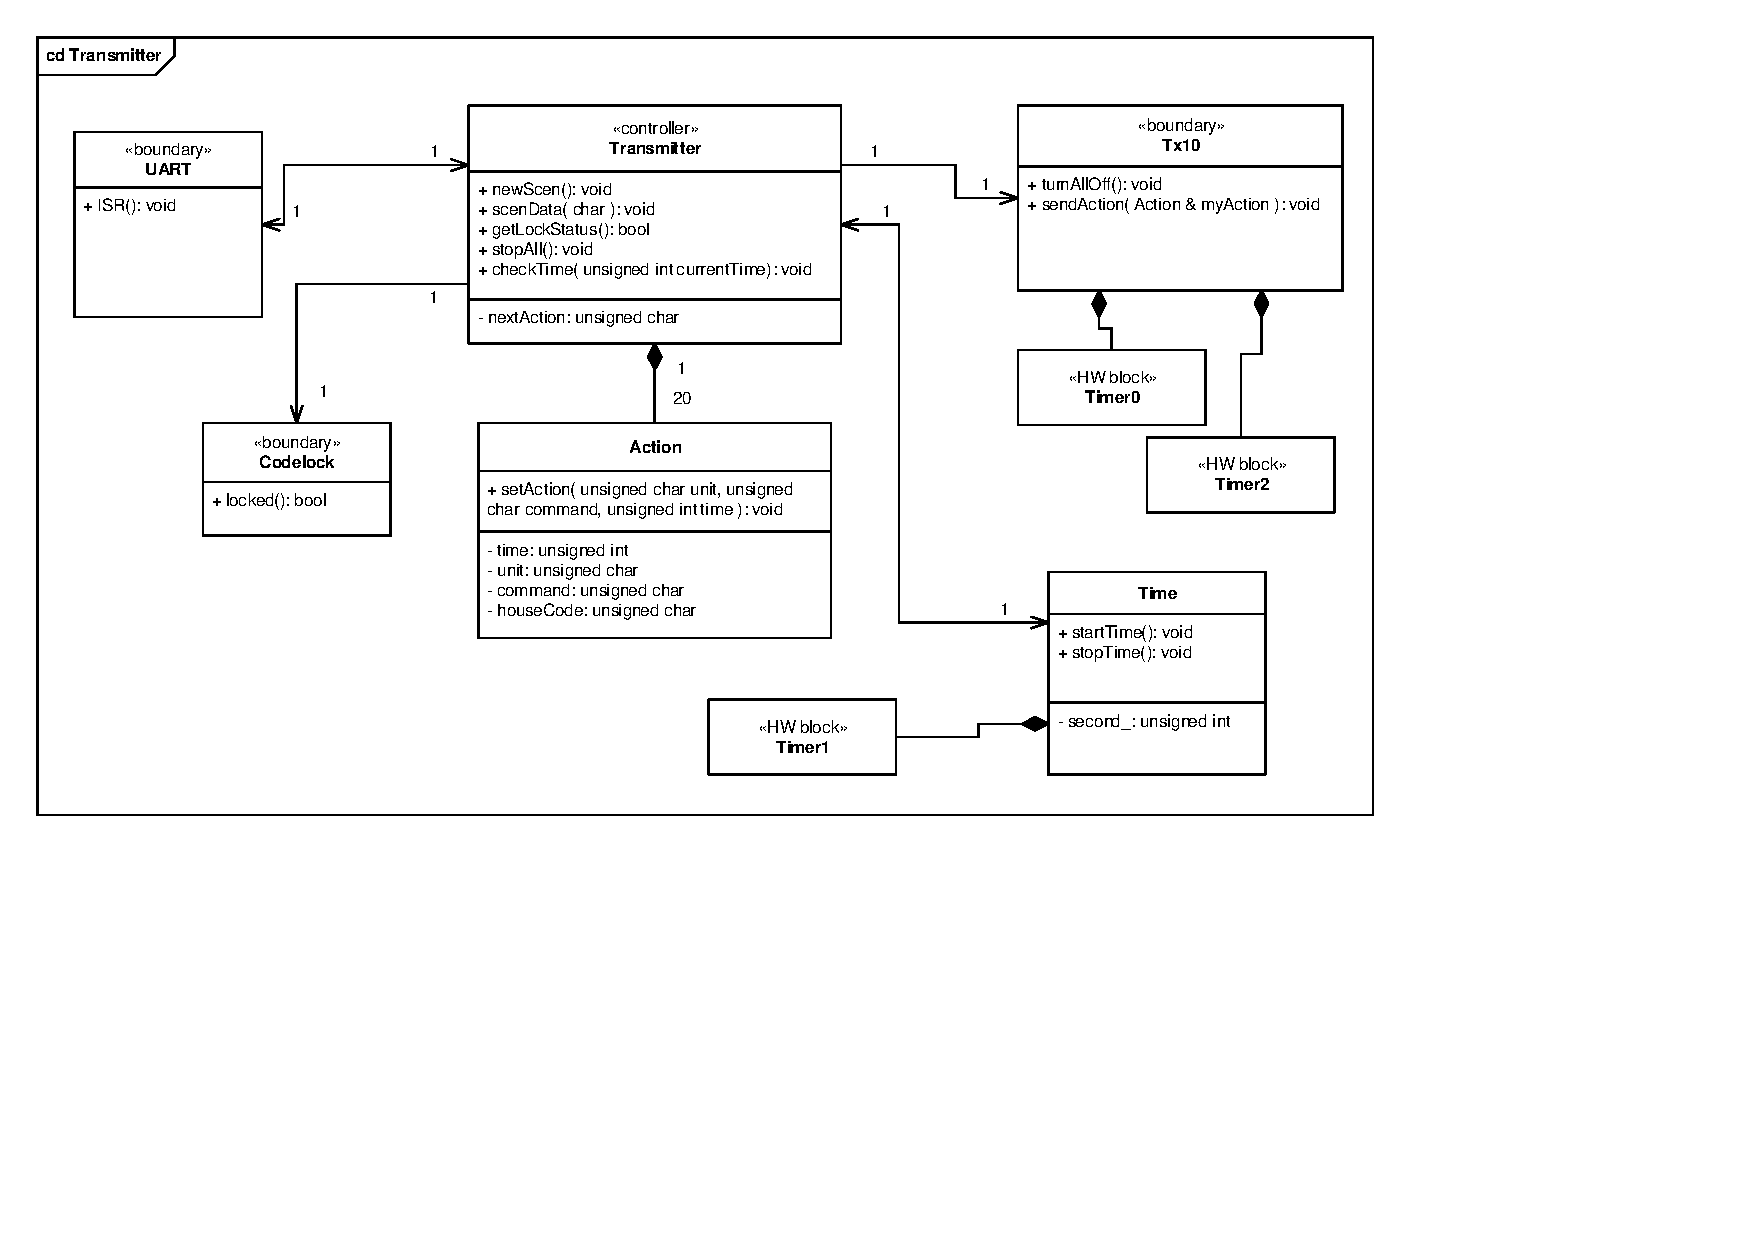
\includegraphics[scale=1,clip=true, trim=38 300 650 203]{Systemarkitektur/diagrammer/Transmitter_Klassediagram} %L B R T - HUSKE DET
\end{figure}

\begin{table}[h]
\begin{tabularx}{\textwidth}{p{0.6 cm} l X} %\hline
\multicolumn{3}{l}{\textbf{unlocked}}\\
& Operation: & %Skriv tekst herunder
\texttt{bool unlocked( void )}
\\ & Parametre: & %Skriv tekst herunder
ingen parametre
\\ & Returværdi: & %Skriv tekst herunder
\texttt{TRUE} hvis den er åben. \texttt{FALSE} hvis den ikke er åben.
\\ & Beskrivelse: & %Skriv tekst herunder
Tjekker om koden er tastet rigtigt ind på vores DE2 board.
\\ \end{tabularx}
\end{table}

\subsection{Time (Kasper)}

\begin{figure}[h]
\centering
\includegraphics[scale=1,clip=true, trim=503 213 195 250]{Systemarkitektur/diagrammer/Transmitter_KlasseDiagram} %L B R T - HUSKE DET
\end{figure}

\begin{table}[h]
\begin{tabularx}{\textwidth}{p{0.6 cm} l X} %\hline
\multicolumn{3}{l}{\textbf{Time}}\\
& Operation: & %Skriv tekst herunder
\texttt{Void Time( )}
\\ & Parametre: & %Skriv tekst herunder
-
\\ & Returværdi: & %Skriv tekst herunder
- 
\\ & Beskrivelse: & %Skriv tekst herunder
-initialisere timer 1 til at interupt hvert sekund.
\\ \end{tabularx}
\end{table}

\clearpage

\begin{table}[h]
\begin{tabularx}{\textwidth}{p{0.6 cm} l X} %\hline
\multicolumn{3}{l}{\textbf{startTime}}\\
& Operation: & %Skriv tekst herunder
\texttt{Void startTime ( void )}
\\ & Parametre: & %Skriv tekst herunder
-
\\ & Returværdi: & %Skriv tekst herunder
- 
\\ & Beskrivelse: & %Skriv tekst herunder
-starter tidstælling på timeren. Tiden tælles op hvert minut.
\\ \end{tabularx}
\end{table}

\begin{table}[h]
\begin{tabularx}{\textwidth}{p{0.6 cm} l X} %\hline
\multicolumn{3}{l}{\textbf{stopTime}}\\
& Operation: & %Skriv tekst herunder
\texttt{Void stopTime ( void )}
\\ & Parametre: & %Skriv tekst herunder
-
\\ & Returværdi: & %Skriv tekst herunder
- 
\\ & Beskrivelse: & %Skriv tekst herunder
-stopper tidstælling på timeren.
\\ \end{tabularx}
\end{table}


\begin{table}[h]
\begin{tabularx}{\textwidth}{p{0.6 cm} l X} %\hline
\multicolumn{3}{l}{\textbf{operator++}}\\
& Operation: & %Skriv tekst herunder
\texttt{operator++()}
\\ & Parametre: & %Skriv tekst herunder
-
\\ & Returværdi: & %Skriv tekst herunder
- 
\\ & Beskrivelse: & %Skriv tekst herunder
-inkremere atributten second med 1.
\\ \end{tabularx}
\end{table}

\begin{table}[h]
\centering
\begin{tabularx}{13 cm}{|l |X|} \hline
Attribut & Beskrivelse \\ \hline
unsigned int second & indeholder tiden i sekunder. \\ \hline
\end{tabularx}
\end{table}

\clearpage

\subsection{Transmitter (Kristian S.)}

\begin{figure}[h]
\centering
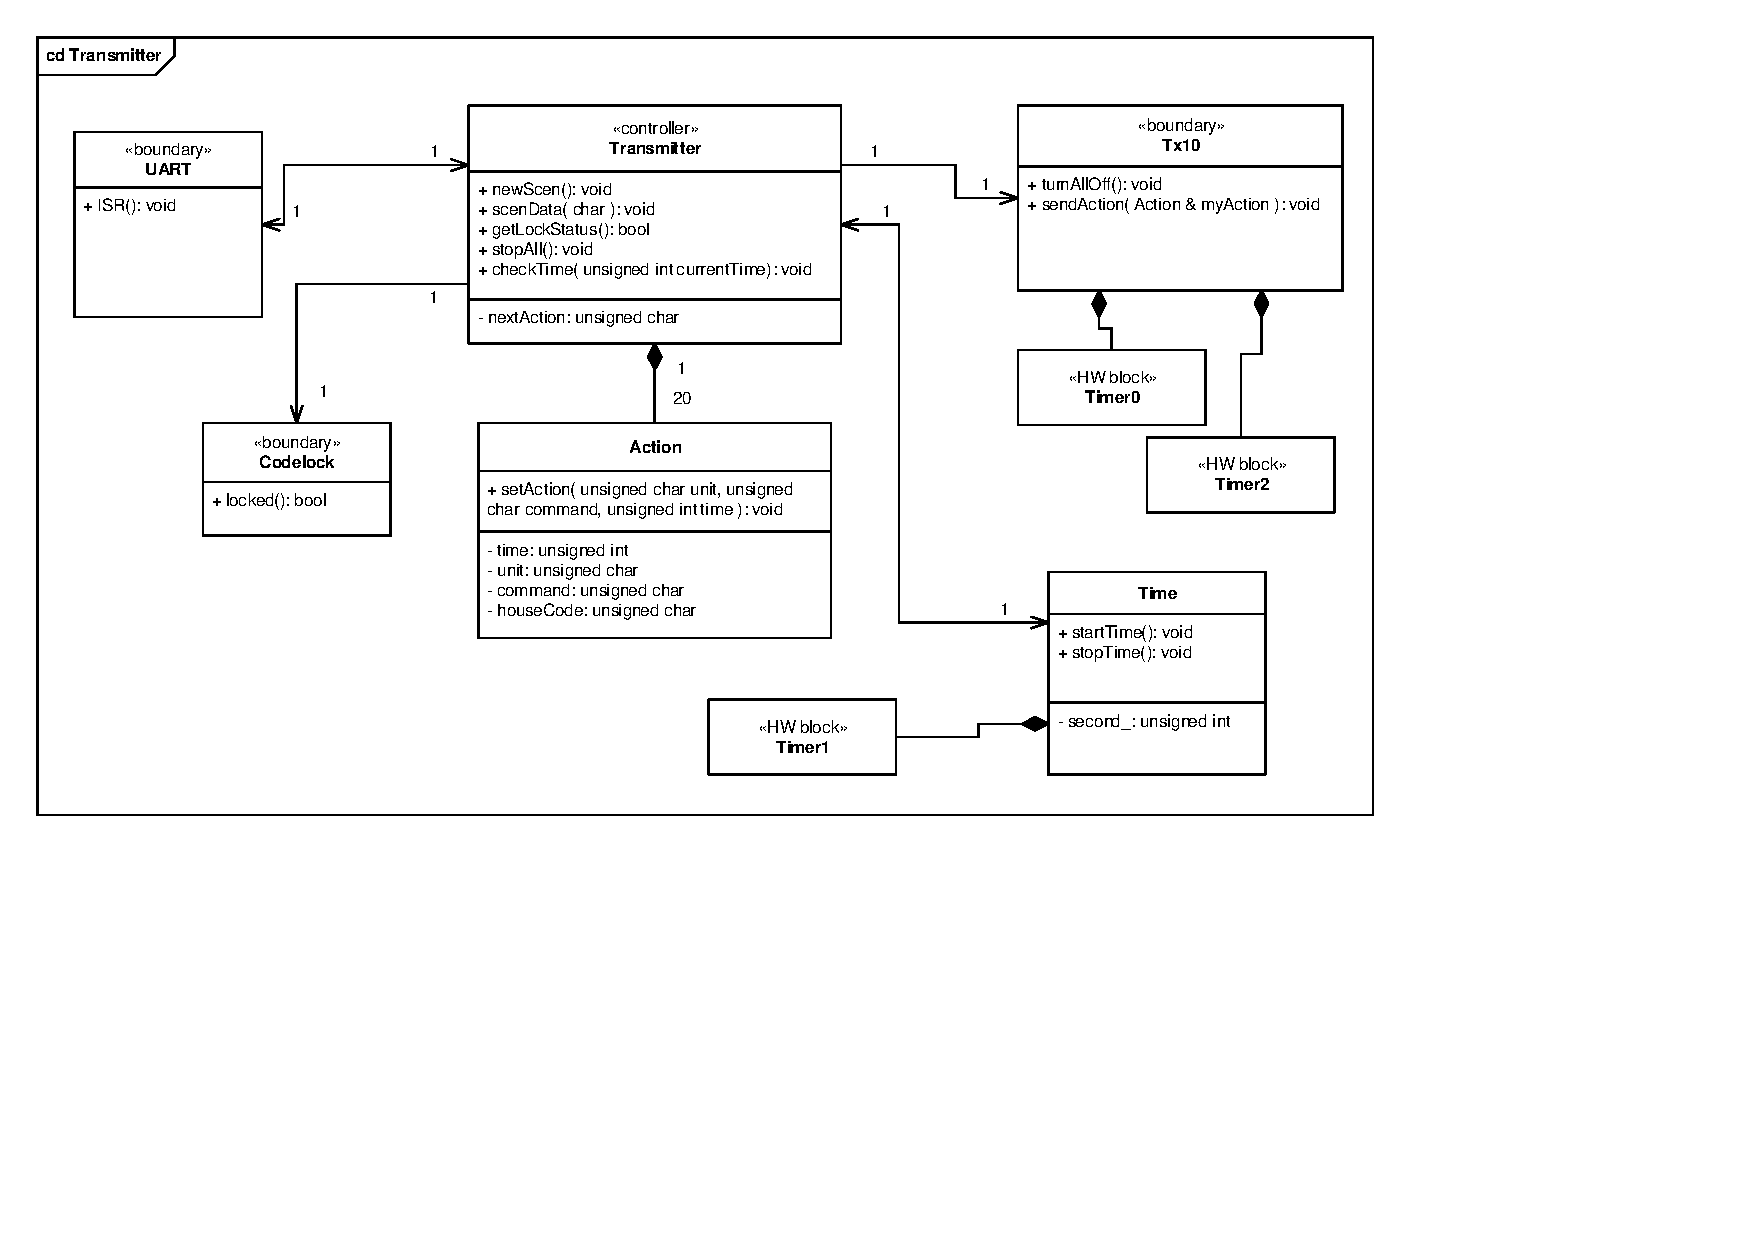
\includegraphics[scale=1,clip=true, trim=225 429 438 50]{Systemarkitektur/diagrammer/Transmitter_Klassediagram} %L B R T - HUSKE DET
\end{figure}

\begin{table}[h]
\begin{tabularx}{\textwidth}{p{0.6 cm} l X} %\hline
\multicolumn{3}{l}{\textbf{\texttt{newScen}}}\\
& Operation: &
\texttt{void newScen( void )}
\\ & Parametre: & %Skriv tekst herunder
-
\\ & Returværdi: & %Skriv tekst herunder
-
\\ & Beskrivelse: & %Skriv tekst herunder
Stopper det igangværende scenarie og sætter nextAction til 0.
\\ \end{tabularx}
\end{table}

\begin{table}[h]
\begin{tabularx}{\textwidth}{p{0.6 cm} l X} %\hline
\multicolumn{3}{l}{\textbf{\texttt{scenData}}}\\
& Operation: &
\texttt{void ScenData( char )}
\\ & Parametre: & %Skriv tekst herunder
\texttt{char}: Indeholder enten information om enhed, kommando eller tidpunkt.
\\ & Returværdi: & %Skriv tekst herunder
$-$
\\ & Beskrivelse: & %Skriv tekst herunder
Methoden har ansvaret for at indsætte char'en i det pågældende aktions-objekt, se UART protokol side \pageref{prot_UART}.
\\ \end{tabularx}
\end{table}

\begin{table}[h]
\begin{tabularx}{\textwidth}{p{0.6 cm} l X} %\hline
\multicolumn{3}{l}{\textbf{\texttt{getLockStatus}}}\\
& Operation: &
\texttt{bool getLockStatus( void )}
\\ & Parametre: & %Skriv tekst herunder
$-$
\\ & Returværdi: & %Skriv tekst herunder
\texttt{bool} : \texttt{TRUE} hvis kodelåsen er indtastet korrekt, \texttt{FALSE} hvis den ikke er.
\\ & Beskrivelse: & %Skriv tekst herunder
Methoden har ansvaret for status angående kodelåsen.
\\ \end{tabularx}
\end{table}

\clearpage

\begin{table}[h]
\begin{tabularx}{\textwidth}{p{0.6 cm} l X} %\hline
\multicolumn{3}{l}{\textbf{\texttt{stopAll}}}\\
& Operation: &
\texttt{void stopAll( void )}
\\ & Parametre: & %Skriv tekst herunder
$-$
\\ & Returværdi: & %Skriv tekst herunder
$-$
\\ & Beskrivelse: & %Skriv tekst herunder
Methoden har ansvaret for at stoppe det igangværende scenarie og at slukke alle tilkoblede enheder, ved at sende stop-kommandoen ud på Tx10, se X10 protokol side \pageref{prot_x10}.
\\ \end{tabularx}
\end{table}

\begin{table}[h]
\begin{tabularx}{\textwidth}{p{0.6 cm} l X} %\hline
\multicolumn{3}{l}{\textbf{\texttt{checkTime}}}\\
& Operation: &
\texttt{void checkTime( unsigned int )}
\\ & Parametre: & %Skriv tekst herunder
\texttt{unsigned int} : Nuværende tid i minutter fra Time-klassen.
\\ & Returværdi: & %Skriv tekst herunder
$-$
\\ & Beskrivelse: & %Skriv tekst herunder
Methoden bliver kaldt fra TimeKlassen hver 5. sekund og er ansvarlig for om den næste aktion skal afvikles. Dette sker kun hvis den givende tid er lig med den næste aktions tid.
\\ \end{tabularx}
\end{table}


\subsection{Transmitter UART (Kasper)}

\begin{figure}[h]
\centering
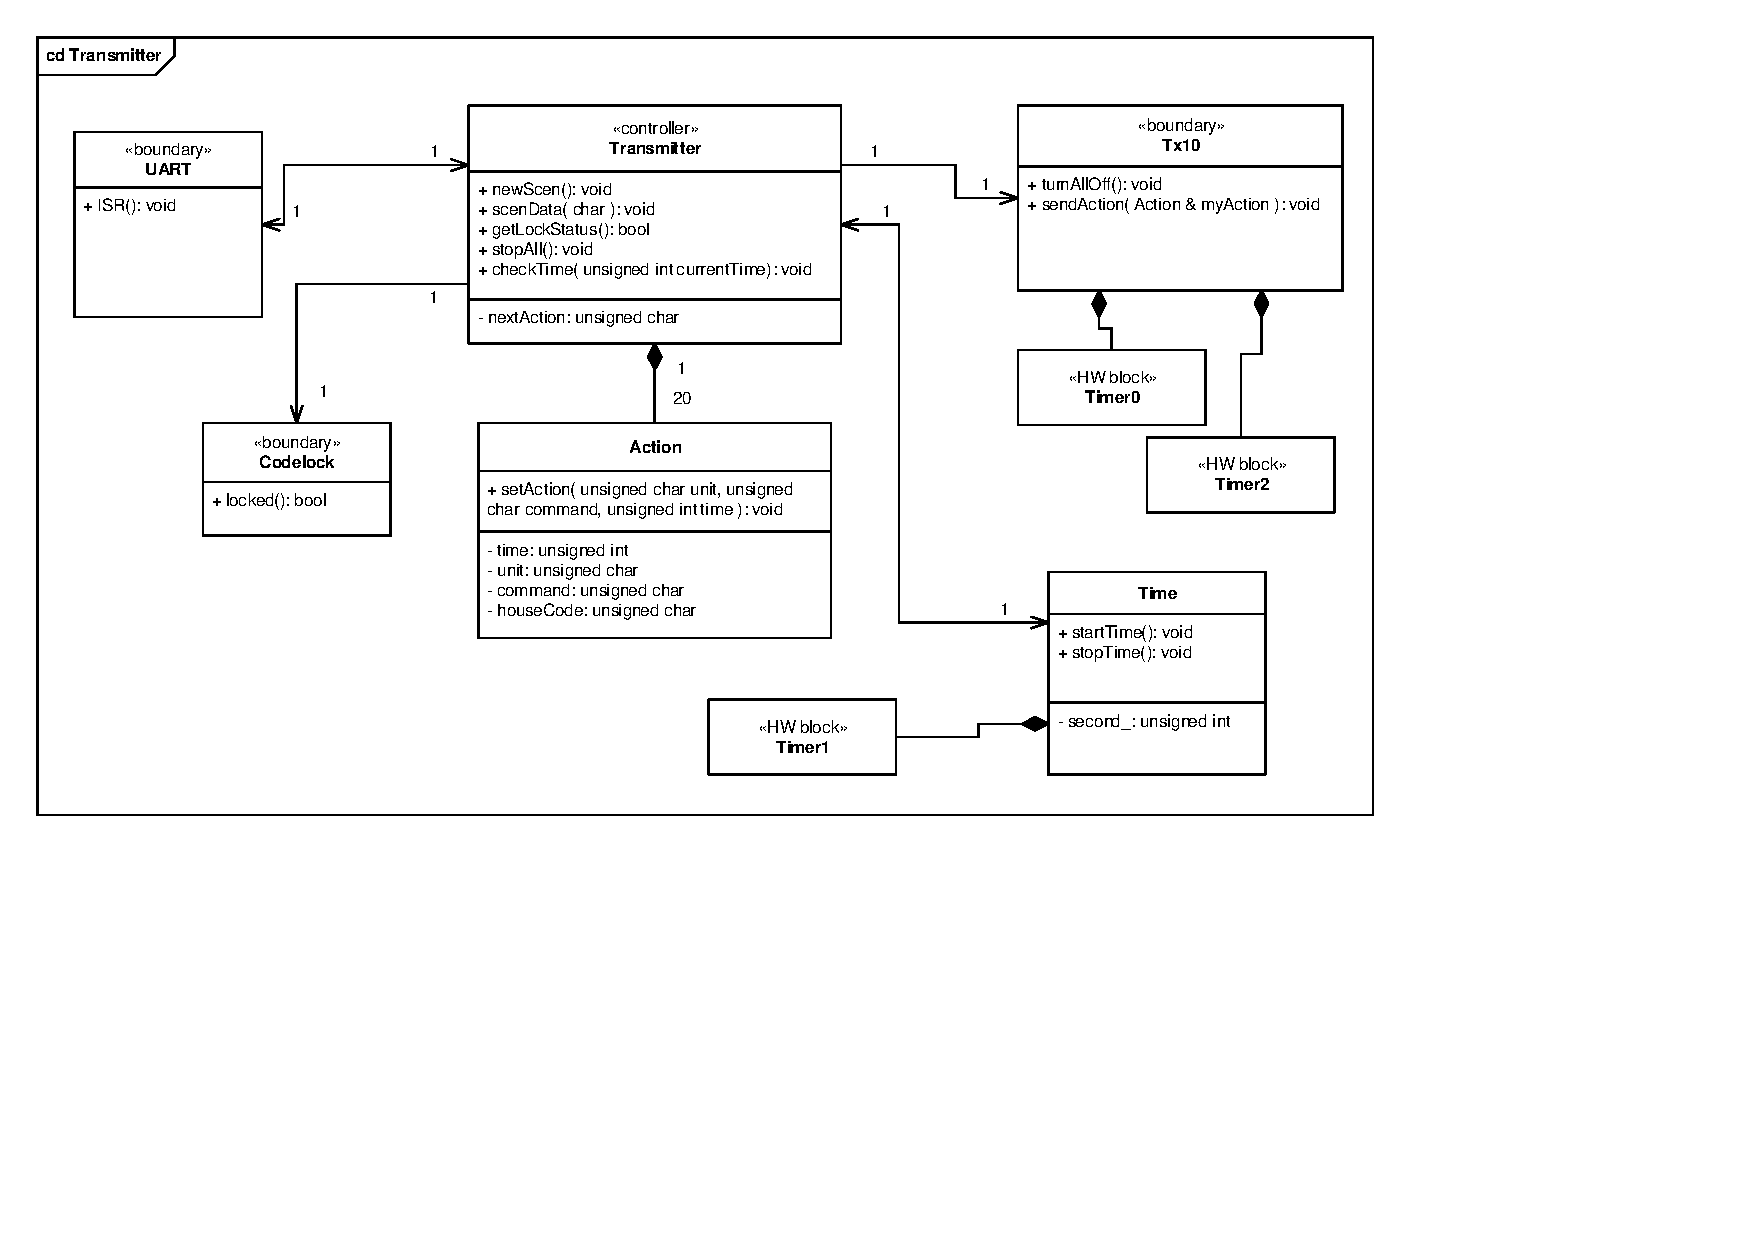
\includegraphics[scale=1,clip=true, trim=25 433 715 60]{Systemarkitektur/diagrammer/Transmitter_Klassediagram} %L B R T - HUSKE DET
\end{figure}

\begin{table}[h]
\begin{tabularx}{\textwidth}{p{0.6 cm} l X} %\hline
\multicolumn{3}{l}{\textbf{constructor}}\\
& Operation: & %Skriv tekst herunder
\texttt{UART} 
\\ & Parametre: & %Skriv tekst herunder
-
\\ & Returværdi: & %Skriv tekst herunder
- 
\\ & Beskrivelse: & %Skriv tekst herunder
opsætter forbindelse på RX og TX til UART, sætter op til brug af interupt.
\\ \end{tabularx}
\end{table}

\clearpage

\begin{table}[h]
\begin{tabularx}{\textwidth}{p{0.6 cm} l X} %\hline
\multicolumn{3}{l}{\textbf{ISR}}\\
& Operation: & %Skriv tekst herunder
\texttt{ISR()} 
\\ & Parametre: & %Skriv tekst herunder
-
\\ & Returværdi: & %Skriv tekst herunder
- 
\\ & Beskrivelse: & %Skriv tekst herunder
Ved interupt på UARTen går transmitteren i 'read mode'. Hvis UART'en læser et L som første char, tjekkes Lockstatus på kodelåsen og returneres til PCen. Hvis et N læses går UARTEN i 'receiving mode' og begynder at aflæse data på reciever pinen. se ref. (state-machine transmitter UART), for lagring af modtagne data. Hvis S modtages sættes transmitteren til 'stop mode'.
\\ \end{tabularx}
\end{table}


\subsection{Tx10 (Kristian T.)}

\begin{figure}[h]
\centering
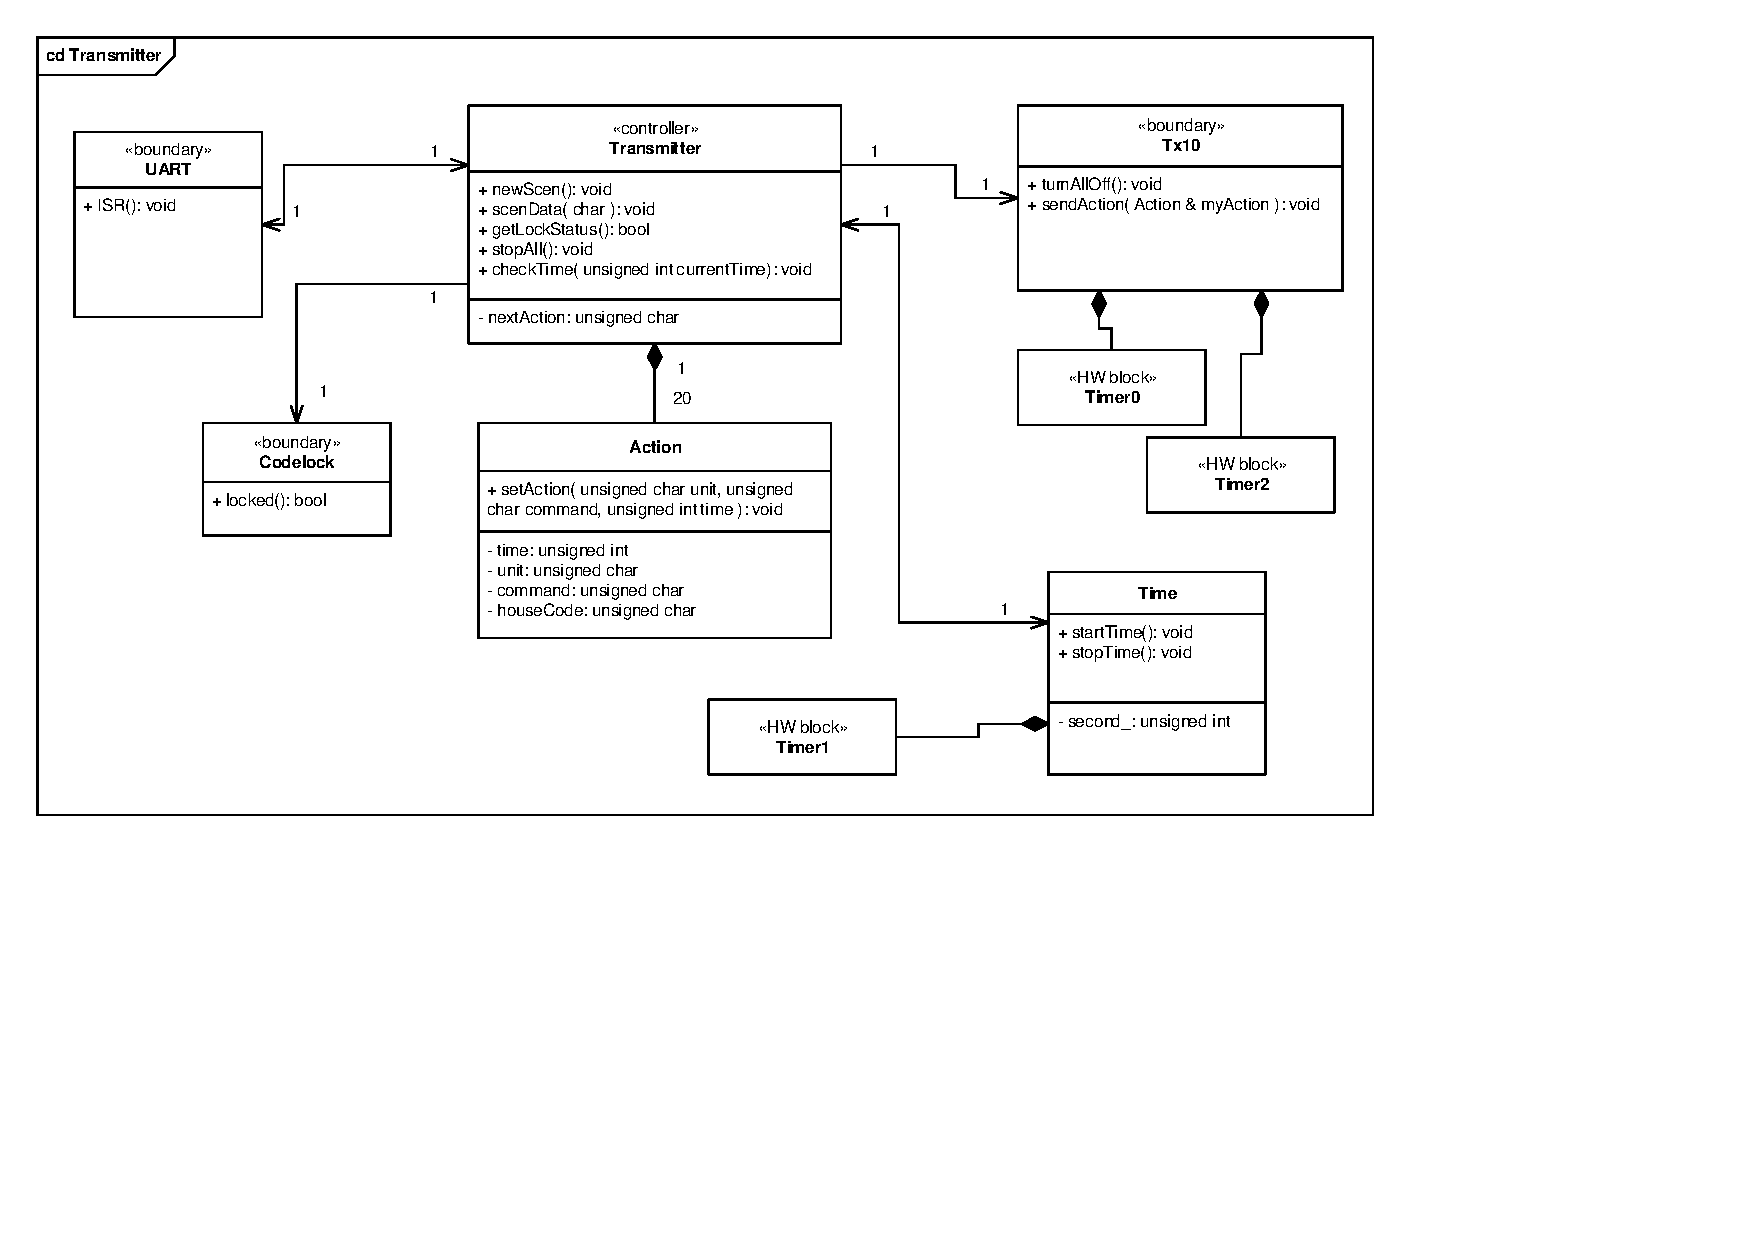
\includegraphics[scale=1,clip=true, trim=488.69 455 197 50]{Systemarkitektur/diagrammer/Transmitter_Klassediagram} %L B R T - HUSKE DET
\end{figure}

%turnAllOff
\begin{table}[h]
\begin{tabularx}{\textwidth}{p{0.6 cm} l X} %\hline
\multicolumn{3}{l}{\textbf{turnAllOff}}\\
& Operation: & %Skriv tekst herunder
\texttt{void turnAllOff()}
\\ & Parametre: & %Skriv tekst herunder
-
\\ & Returværdi: & %Skriv tekst herunder
-
\\ & Beskrivelse: & %Skriv tekst herunder
Når denne metode kaldes, sendes slukke-kommandoer ud til samtlige enheder på netværket via \texttt{sendAction()}.
\\ \end{tabularx}
\end{table}

%sendAction
\begin{table}[h]
\begin{tabularx}{\textwidth}{p{0.6 cm} l X} %\hline
\multicolumn{3}{l}{\textbf{sendAction}}\\
& Operation: & %Skriv tekst herunder
\texttt{void sendAction( Action \& myAction )} 
\\ & Parametre: & %Skriv tekst herunder
Modtager en reference til det pågældende objekt af klassen \texttt{Action}, som skal eksekveres.
\\ & Returværdi: & %Skriv tekst herunder
-
\\ & Beskrivelse: & %Skriv tekst herunder
Skal ved hjælp af protokollen for kommunikation over X.10 afsende kommandoer. Der skal sendes én bit hver anden interrupt/nulgennemgang på \texttt{PD2 (INT0)} (interrupt i toggle mode). Ved hver bit skal der ved det efterfølgende interrupt sendes det modsatte af det foregående. Hver gang et 1-tal skal sendes, skal dette være HIGH i 1 ms fra nulgennemgangen/interruptet.
\\ \end{tabularx}
\end{table}

\clearpage

%constructor
\begin{table}[h]
\begin{tabularx}{\textwidth}{p{0.6 cm} l X} %\hline
\multicolumn{3}{l}{\textbf{Constructor}}\\
& Operation: & %Skriv tekst herunder
\texttt{Tx10( void ) }
\\ & Parametre: & %Skriv tekst herunder
Ingen
\\ & Beskrivelse: & %Skriv tekst herunder
Skal initiere \texttt{Timer0} samt interrupt på \texttt{PD2 (INT0)}, men dog ikke aktivere disse.
\\ \end{tabularx}
\end{table}

\section{Receiver blokken}

\subsection{Lampe (David)}

\begin{figure}[h]
\centering
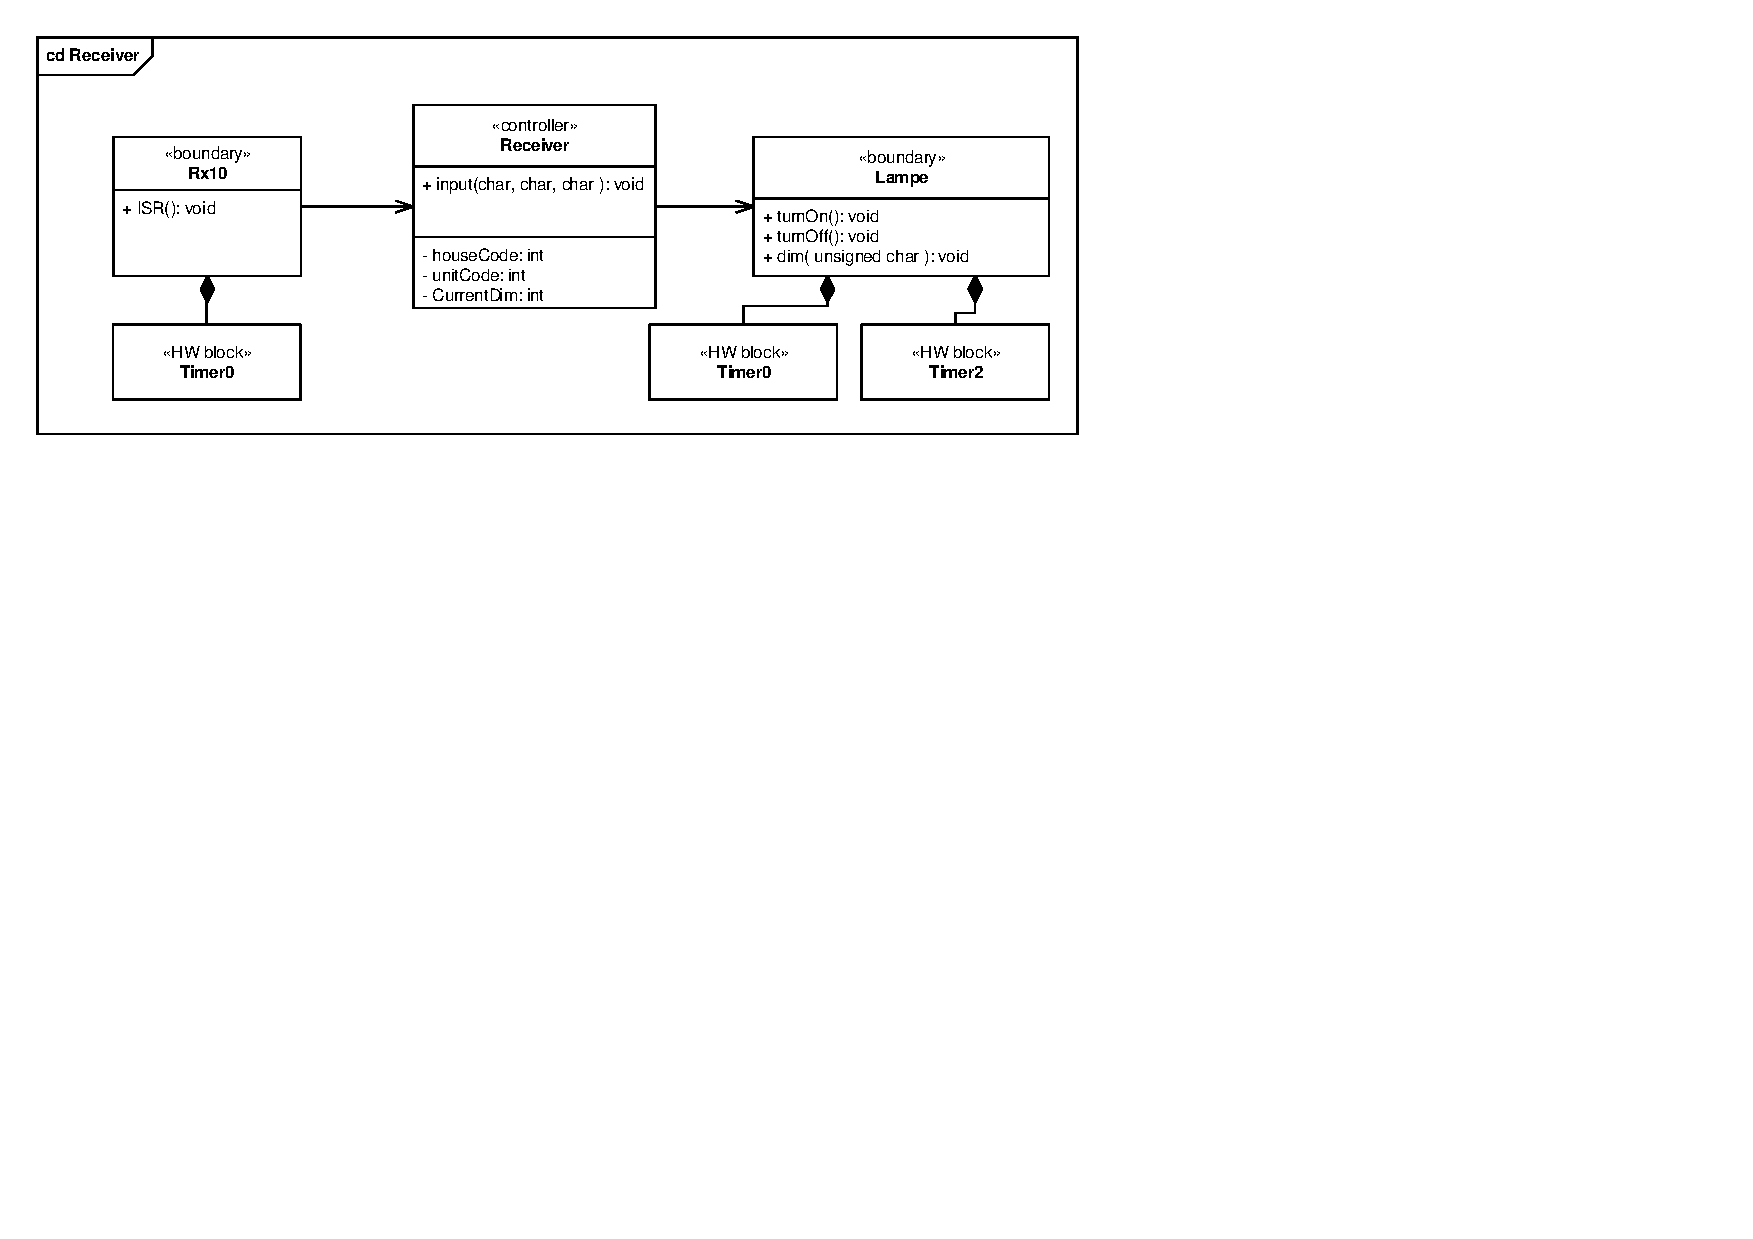
\includegraphics[scale=1,clip=true, trim=361.8 462 335 50]{Systemarkitektur/diagrammer/Receiver_KlasseDiagram} %L B R T - HUSKE DET
\end{figure}

\begin{table}[h]
\begin{tabularx}{\textwidth}{p{0.6 cm} l X} %\hline

%turnOn
\multicolumn{3}{l}{\textbf{turnOn}}\\
& Operation: & %Skriv tekst herunder
\texttt{void turnOn( void )}
\\ & Parametre: & %Skriv tekst herunder
Ingen.
\\ & Returværdi: & %Skriv tekst herunder
Ingen.
\\ & Beskrivelse: & %Skriv tekst herunder
Sætter PWM for lampen til 100\%.

\\ \end{tabularx}
\end{table}

%turnOff
\begin{table}[h]
\begin{tabularx}{\textwidth}{p{0.6 cm} l X} %\hline

\multicolumn{3}{l}{\textbf{turnOff}}\\
& Operation: & %Skriv tekst herunder
\texttt{void turnOff( void )}
\\ & Parametre: & %Skriv tekst herunder
Ingen
\\ & Returværdi: & %Skriv tekst herunder
Ingen
\\ & Beskrivelse: & %Skriv tekst herunder
Sætter PWM for lampen til 0\%.

\\ \end{tabularx}
\end{table}

\clearpage

%dim
\begin{table}[h]
\begin{tabularx}{\textwidth}{p{0.6 cm} l X} %\hline

\multicolumn{3}{l}{\textbf{dim}}\\
& Operation: & %Skriv tekst herunder
\texttt{void dim ( char )}
\\ & Parametre: & %Skriv tekst herunder
Modtager en char med en char med den ønskede dimnings værdi.
\\ & Returværdi: & %Skriv tekst herunder
Ingen
\\ & Beskrivelse: & %Skriv tekst herunder
Modtager en char som har en værdi mellem 0 og til og med 9, hvor 0 = 5\%, 1 = 15\% osv. Skal herefter ændre pulsbredden på det ben der er forbundet til lampen i forhold til den ovenfor angivne procent.
\\ \end{tabularx}
\end{table}

\subsection{Receiver (David)}

\begin{figure}[h]
\centering
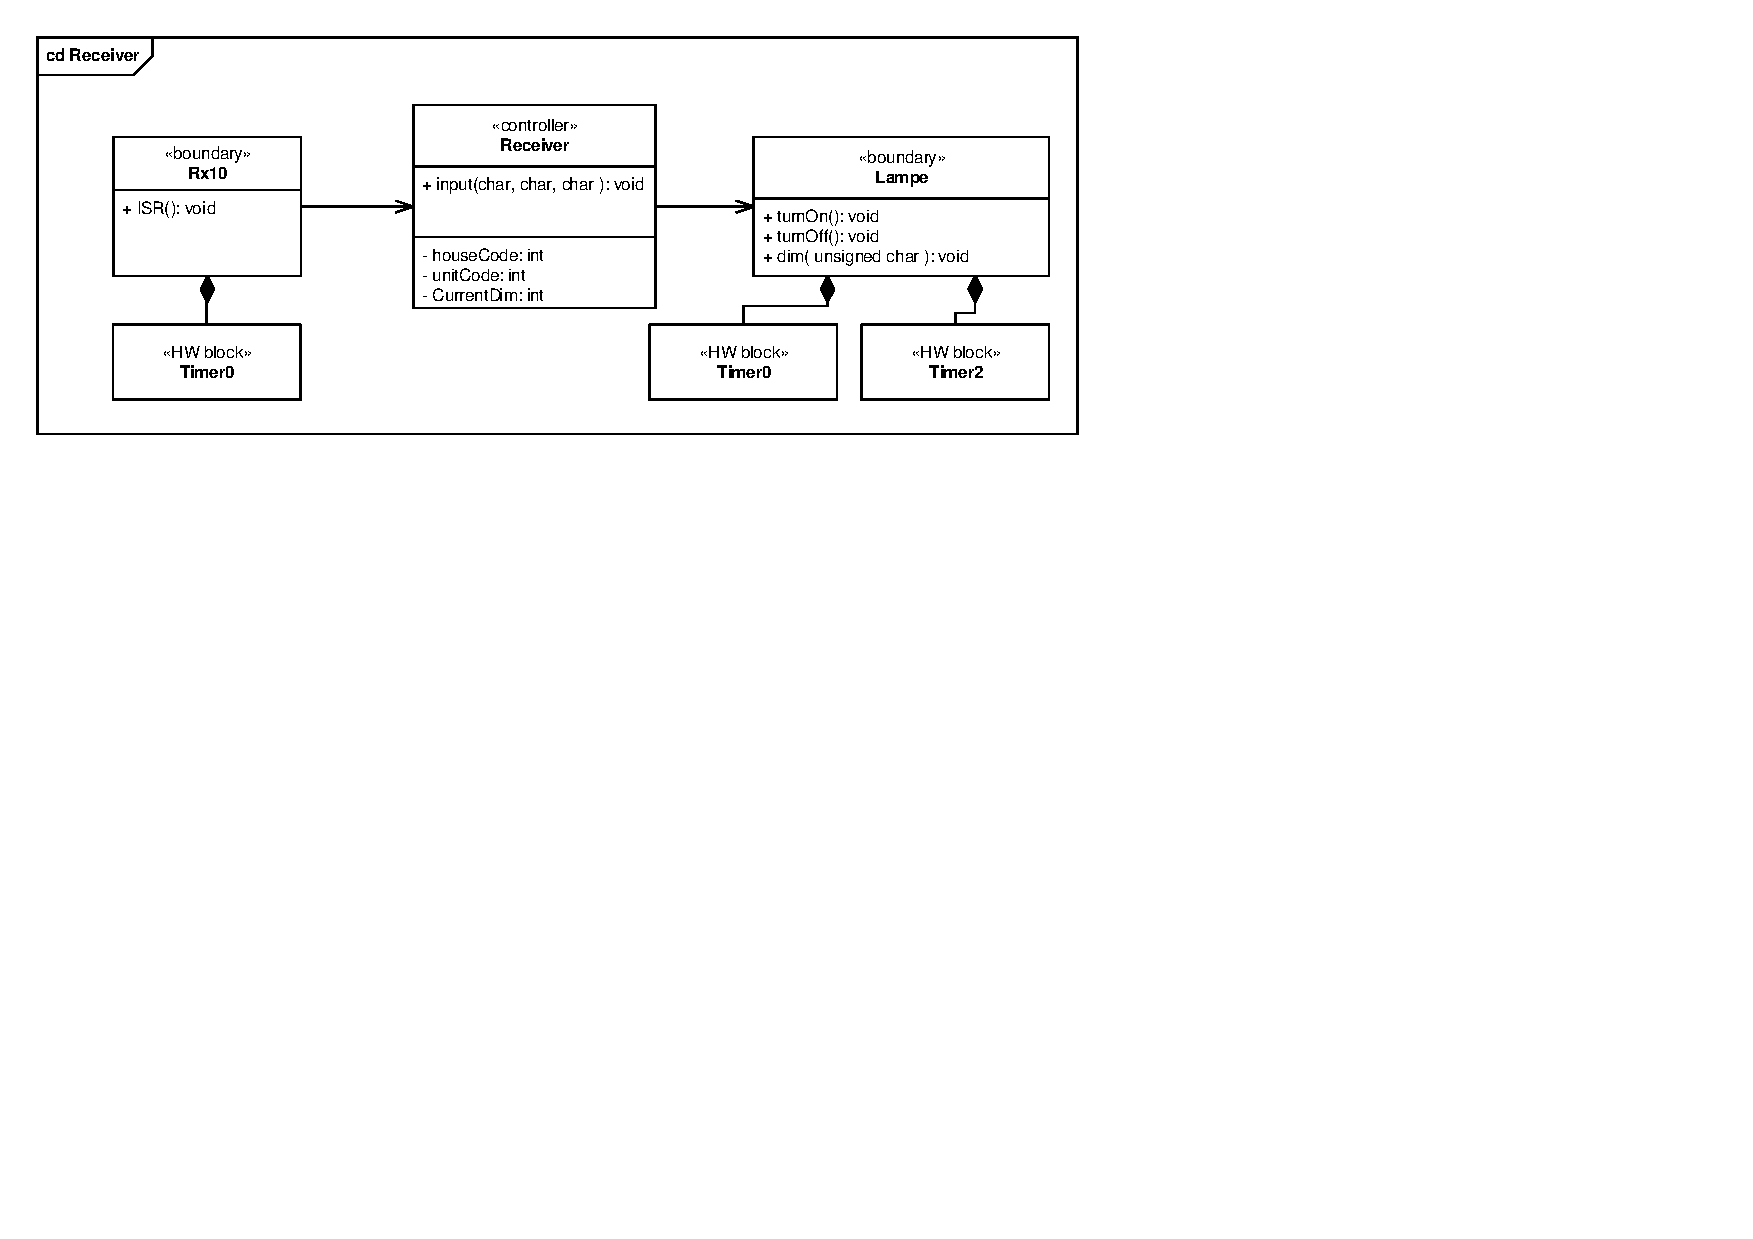
\includegraphics[scale=1,clip=true, trim=198 440 527 50]{Systemarkitektur/diagrammer/Receiver_KlasseDiagram} %L B R T - HUSKE DET
\end{figure}

\begin{table}[h]
\begin{tabularx}{\textwidth}{p{0.6 cm} l X} %\hline
\multicolumn{3}{l}{\textbf{Receiver}}\\
& Operation: & %Skriv tekst herunder
void input( char ) 
\\ & Parametre: & %Skriv tekst herunder
Modtager en char fra X.10 som bruges til at finde om lampen skal. Tænde, slukke, dime op, eller dime ned.
\\ & Returværdi: & %Skriv tekst herunder
ingen retur værdi. 
\\ & Beskrivelse: & %Skriv tekst herunder
Controller for receiveren. Holder styr på lampen nuværerne dimning samt dens houseCode og unitCode.
\\ \end{tabularx}
\end{table}

\begin{table}[h]
\centering
\begin{tabularx}{13 cm}{|l |X|} \hline
Attribut & Beskrivelse \\ \hline

houseCode & Indeholder hus koden for denne Receiver \\ \hline
unitCode  & Indeholder unit koden for denne Receiver \\ \hline
CurrentDim & Den nuværerne dim værdi. \\ \hline

\end{tabularx}
\end{table}

\clearpage

\subsection{Rx10 (Kristian T.)}

\begin{figure}[h]
\centering
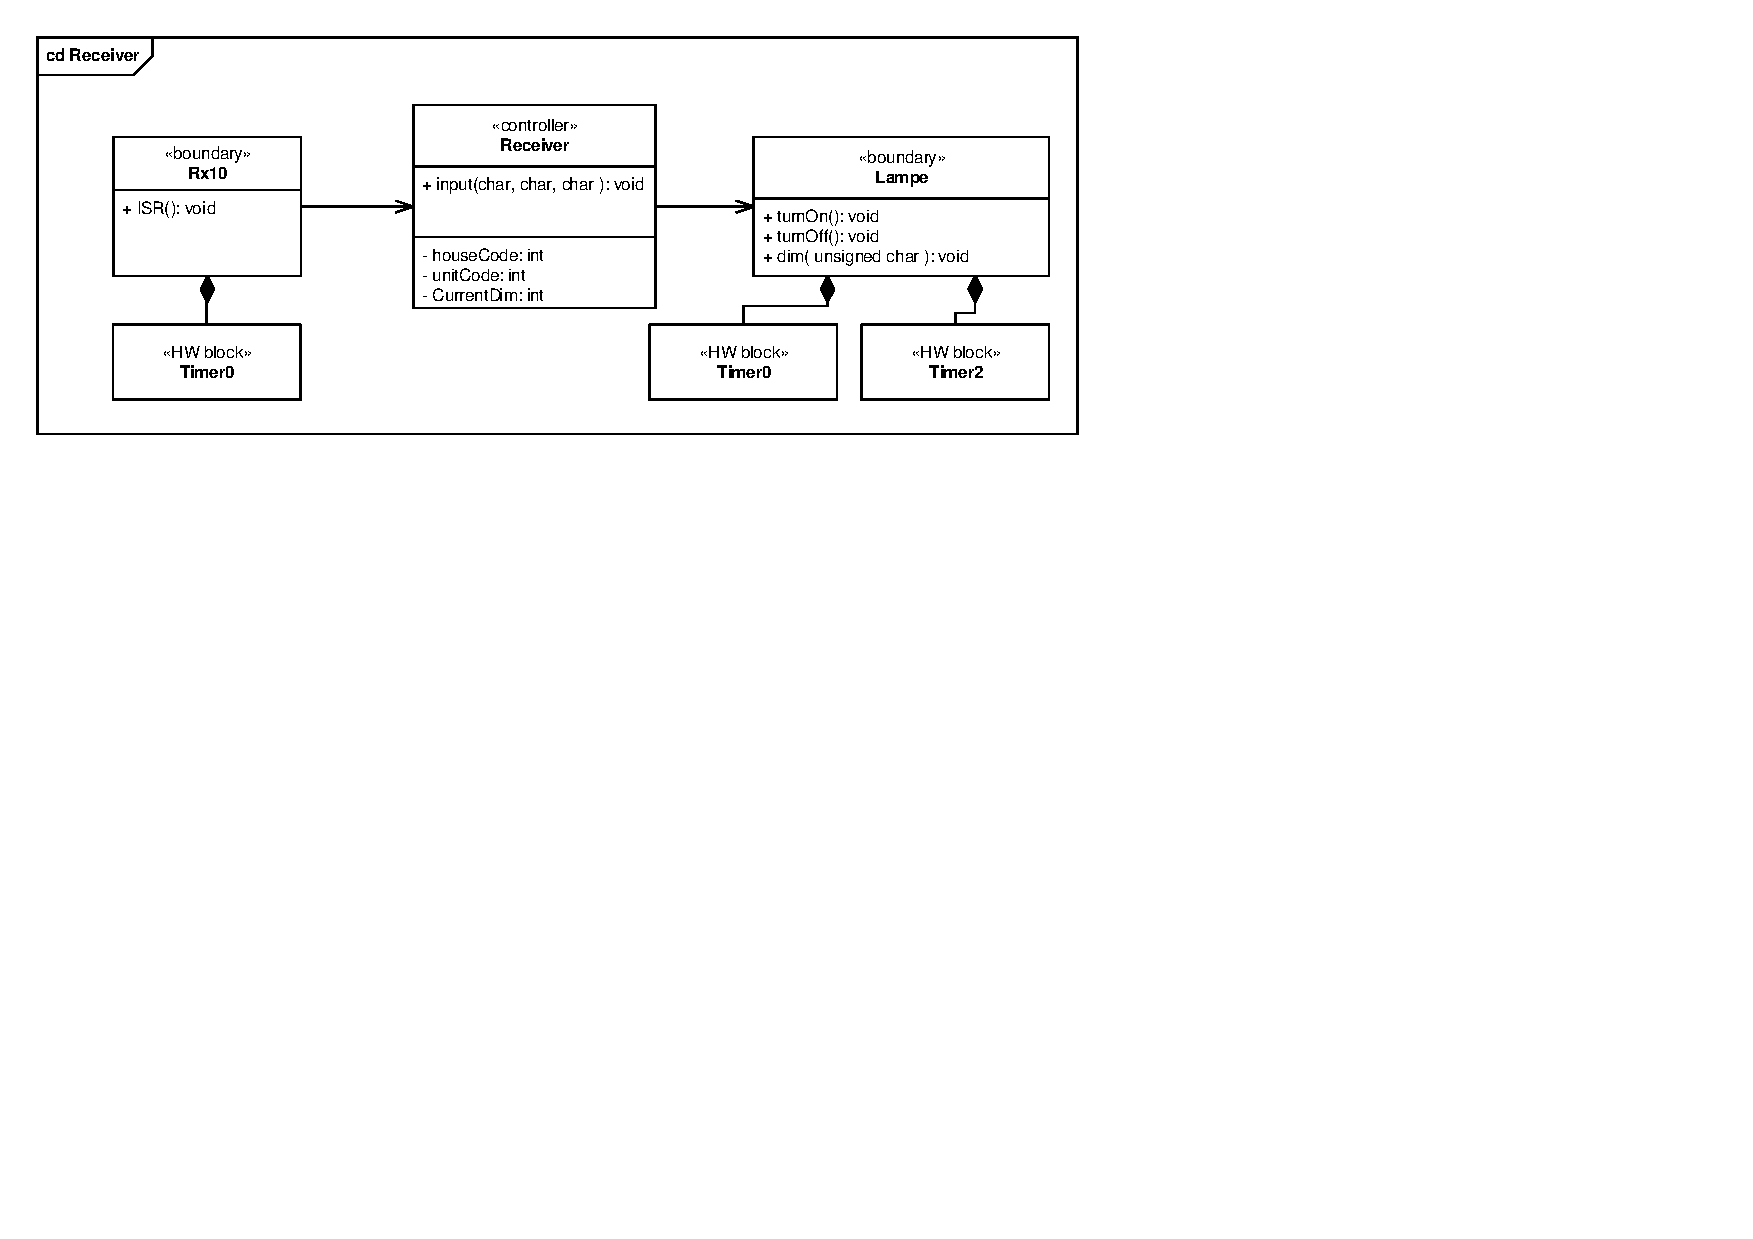
\includegraphics[scale=1,clip=true, trim=38 462 697 66]{Systemarkitektur/diagrammer/Receiver_KlasseDiagram} %L B R T - HUSKE DET
\end{figure}

%ISR
\begin{table}[h]
\begin{tabularx}{\textwidth}{p{0.6 cm} l X} %\hline
\multicolumn{3}{l}{\textbf{ISR}}\\
& Operation: & %Skriv tekst herunder
\texttt{ISR( INT0\_vect )}
\\ & Parametre: & %Skriv tekst herunder
Denne servicerutine er indbygget i Atmega32's IO bibliotek og modtager ingen parametre \cite{lib:AtMega32sum}.
\\ & Beskrivelse: & %Skriv tekst herunder
Denne funktion kaldes ved interrupts på \texttt{PD2 INT0} og skal være \texttt{Friend} af klassen. Ved interrupts skal denne skifte den nuværende værdi på PA0 ind i \texttt{temp}. Der udføres udføres herefter forskellige handlinger afhængigt tilstanden.
\\
\end{tabularx}
\end{table}

%checkData
\begin{table}[h]
\begin{tabularx}{\textwidth}{p{0.6 cm} l X} %\hline
\multicolumn{3}{l}{\textbf{checkData}}\\
& Operation: & %Skriv tekst herunder
\texttt{bool checkData( unsigned char )}
\\ & Parametre: & %Skriv tekst herunder
Modtager 8 nulgennemgange.
\\ & Returværdi: & %Skriv tekst herunder
Returnerer \texttt{TRUE}, hvis de 8 nulgennemgange overholder protokollen for 4 bits og \texttt{FALSE}, hvis den ikke gør.
\\ & Beskrivelse: & %Skriv tekst herunder
Denne metode kontrolleer om en given 4-bit størrelse overholder X.10 protokollen. Der modtages 8 nulgennemgange, som deles op i 4 par. Hvert par udgør 1 bit. For at returnere \texttt{TRUE} skal hvert par bestå af ét 1-tal og ét 0.
\\
\end{tabularx}
\end{table}

%translate
\begin{table}[h]
\begin{tabularx}{\textwidth}{p{0.6 cm} l X} %\hline
\multicolumn{3}{l}{\textbf{translate}}\\
& Operation: & %Skriv tekst herunder
\texttt{unsigned char translate( unsigned char )}
\\ & Parametre: & %Skriv tekst herunder
Modtager en \texttt{char}, som repræsenterer 8 nulgennemgange.
\\ & Returværdi: & %Skriv tekst herunder
Returnerer en \texttt{char} bestående af \texttt{0000} efterfulgt af de 4 bits, som inputtet oversættes til.
\\ & Beskrivelse: & %Skriv tekst herunder
Metoden tager parameteren og oversætter den til 4 bits. For at fylde \texttt{char}'en sættes bit 7-4 til \texttt{0} i returværdien. Bit 3-0 på returværdien sættes til bit 7, 5, 3 og 1 fra parameteren. 
Dvs hvis metoden kaldes med en char \texttt{10011010} vil returværdien være: \texttt{00001011}. 
\\
\end{tabularx}
\end{table}

\begin{table}[h!]
\centering
\begin{tabularx}{13 cm}{|l |X|} \hline
Attribut & Beskrivelse \\ \hline

\texttt{bool start} & Sættes til \texttt{TRUE}, hvis den er igang med at modtage en kommando, ellers sættes den til \texttt{FALSE}. \\ \hline
\texttt{unsigned char count} & Tæller hvor mange nulgennemgange der har været siden sidste hele bit/mønster. \\ \hline
\texttt{unsigned char temp} & Variabel som agerer skifteregister ved modtagelse af nulgennemgange. \\ \hline
\end{tabularx}
\end{table}

\clearpage
\section{Protokoller (Kristian T., Kristian S., David og Kasper)}

\subsection{Protokol for UART}\label{prot_UART}

For kommunikation mellem Transmitter og PC bruges UART med 8 bits bredde. I de to forskellige stadier kan der sendes forskellige ting, under Receiving stadiet skal der sendes: Unit, Command, TimeL, TimeH.

\begin{table} [h]
\centering
\begin{tabular}{|l |l |} \hline 
\multicolumn{2}{|c|}{\textbf{Idle state}} \\ \hline
Mode:      & Value \\ \hline
Lockstatus & L,ret: L\/ U \\
Newscen    & N            \\		 
Stop       & S            \\
\hline
\end{tabular}
\caption{Tilgængelige værdier i 'Idle' state.}
\end{table}

\begin{table} [h]
\centering
\begin{tabular}{|l |l |l | l | l | l| l| l| l|l|l|} \hline
\multicolumn{8}{|c|}{\textbf{Receiving state}} \\ \hline
Unit: & Value && Command: & Value  && Time &  Value       \\ \cline{1-2} \cline{4-5} \cline{7-8}
Arne (L1)     & 'A' && Dim  & 'A' - 'J' &&  bin\_val & 0x0000 - 0x05FF  \\  \cline{7-8} %\cline{1-2} \cline{4-5}
Carl (L2)     & 'C' && Tænd & 'T'    \\	 %\cline{7-8} % \cline{1-2} \cline{4-5}
Per (TV)      & 'P' && Sluk & 'S' & \multicolumn{3}{l}{ } \\ \cline{4-5} % \cline{7-8} \cline{1-2}
Nils (Radio)  & 'N' & \multicolumn{6}{l}{ } \\ \cline{1-2}  %\cline{7-8} %\cline{4-5}
\end{tabular}
\caption{Tilgængelige værdier i 'Receiving' state.}
\end{table}

Fra UARTen på PCen bliver det sendt i rækkefølgen: unit, command, timeLow, timeHigh. Hvor unit er en af de 4 mulige units. Command er en af kommandoerne: T,S eller A til J, hvor A til J er forskellige dimming styrker.
Time sendes opdelt i 3 chars. Første char sender de første 4 bit, kodet således at 0 = ASCII værdien for 0, 1 = ASCII værdien for 1 osv. Dvs at Selve tallet + 48 sendes. Det samme gælder for den næste char, som repræsentere bit 4-7. Den sidste char repræsenterer bit 8-11 af den \texttt{INT}, som indeholder tiden. Dette er den maksimale tid, da det er antallet af minutter på et døgn.
Der bliver sendt med asynkront, 8bit, 1 stopbit, ingen paritet, og en baudrate på 9600.

\clearpage

\subsection{Protokol for X10}\label{prot_x10}

Ved kommunikation med X10, har vi lavet vores egen protokol med inspiration fra AN236 Applicationsnote \cite{lib:AN236}. En bit består af to nulgennemgange, hvor de er hinandens omvendte. Dvs: \texttt{1 = 10} og \texttt{0 = 01}. Udover dette er der et specifikt startmønster \texttt{"1110"} og et specifikt stopmønster \texttt{"1111"}, samt en ventekode \texttt{"000000"}. Hver kommando skal sendes to gange i stræk, adskilt af ventekoden. I Tabel \ref{tbl:x.10pattern} ses hvordan en kommando er opbygget i X10.

\begin{table} [h]
	\centering
    \begin{tabular}{|l|l|l|l|l|l|l|l|l|l|}
    \hline    
    Startcode & 4 bit & 4 bit & 4 bit & waitcode &  4 bit & 4 bit & 4 bit & Stopcode\\ \hline
    1110            & House & Unit & Command & 000000  &   House & Unit  & Command & 1111 \\ \hline
    \end{tabular}
\caption{Mønster for hvordan en kommando sendes via X.10}
\label{tbl:x.10pattern}
\end{table}

4 bit værdien 'House' erstattes med en af nedenstående huskoder. Hvis koden "All off" modtages, kaldes der i hver receiver en off funktion.

\begin{table} [h]
\centering
    \begin{tabular}{|l|l|l|}
    \hline
    House & Value  & Kommentar          \\ \hline
    All off & 0      & Slukker alt        \\ \hline
    Lamps   & 1      & ~                  \\ \hline
    TV      & 2      & ~                  \\ \hline
    Radio   & 3      & ~                  \\ \hline
    Resrved & 4.. 15 & ikke taget i brug. \\ \hline
    \end{tabular}
\caption{Tilgængelige huskoder i X10.}
\end{table}

Ligeledes erstattes 'Unit' med en af de nedenstående enheder:

\begin{table} [h]
\centering
    \begin{tabular}{|l|l|l|}
    \hline
    Unit    & Value   \\ \hline
    Lampe 1 & 1     \\ \hline
    Lampe 2 & 2      \\ \hline
    TV      & 4     \\ \hline
    Radio   & 8     \\ \hline
    \end{tabular}
\caption{Tilgængelige huskoder i X10.}
\end{table}

Hver enhed har hver sit sæt af kommandoer, da vi kun vælger at implementere lamper, er her en liste over kommanoder for lamper:

\begin{table} [h]
\centering
    \begin{tabular}{|l|l|}
    \hline
    CMD\_L    & Value    \\ \hline
    Sluk      & 0        \\ \hline
    Tænd      & 1        \\ \hline
    Dim 5\%   & 2        \\ \hline
    DIm 15\%  & 3        \\ \hline
    sim ...\% & ...      \\ \hline
    Dim 95\%  & 11       \\ \hline
    Reserved  & 12... 15 \\ \hline
    \end{tabular}
\caption{Tilgængelige kommandoer for lamper.}
\end{table}







\section{Porte (Kristian T., Kristian S., David og Kasper)}

\subsubsection{Transmitter}

\begin{itemize}
\item D0 (RXD) \& D1 (TXD): Bruges til at kommunikere via UART med PC blokken.
\item D2 (INT0): Betragtes som \texttt{ZeroCrossDetect: bool} fra Figur \ref{fig:IBDx.10transmit} side \pageref{fig:IBDx.10transmit}.
\item B3 (OC0): Forbindes til \texttt{X.10Data: bitstream}, bruges til at sende data fra transmitter via X10.
\item A0: Henter status fra kodelåsen.
\end{itemize}

\subsubsection{Receiver}

Receiver blokken ejer følgende porte på STK500:
\begin{itemize}
\item D0 (RXD) \& D1 (TXD): Bruges til debugging af Receiveren ved at sende input fra X10 ud via UART.
\item A0: Betragtes som \texttt{X.10Data: bitstream} fra Figur \ref{fig:IDBx.10lys} på side \pageref{fig:IDBx.10lys}.
\item D2 (INT0): Betragtes som \texttt{ZeroCrossDetect: bool} fra Figur \ref{fig:IDBx.10lys} side \pageref{fig:IDBx.10lys}.
\item B3 (OC0): Forbindes til \texttt{LightCntrl: CntrlPWM} fra ovenstående figur.
\end{itemize}

\clearpage
\begin{landscape}
\section{Statemachines (Kristian S. og David)}

\subsubsection{Statemachine over UART/transmitter }

\begin{figure}[h]
\centering
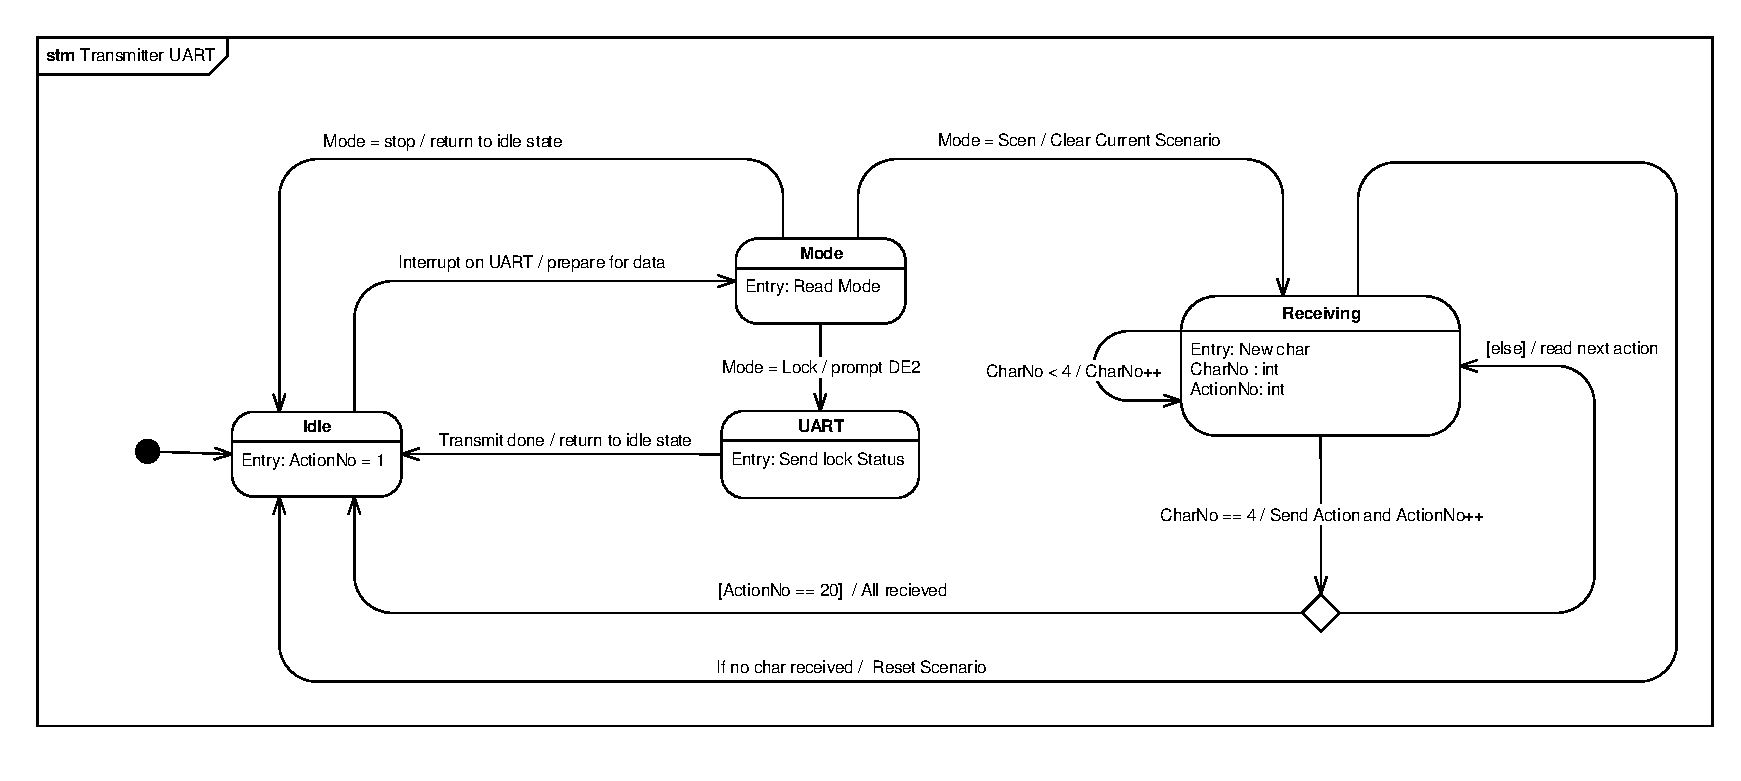
\includegraphics[width=\textheight + 190pt,clip=true, trim=18 18 10 18]{Systemarkitektur/diagrammer/Stm_transmitter_UART} %L B R T - HUSKE DET
\end{figure}

Statemachinen viser Transmitteren's tilstande når PC'en sender data over UART'en. Den første block Mode er et af følgende: Lock, Stop, og Scen(Scenarie). Hvis Scen er sendt, gør transmitter klar til at modtage flere data om det nye scenarie. Efter alt data er modtaget, starter transmitteren det nye scenariet og returner til idle tilstanden.

\newpage

\subsubsection{Statemachine over X.10/transmitter }

\begin{figure}[h]
\centering
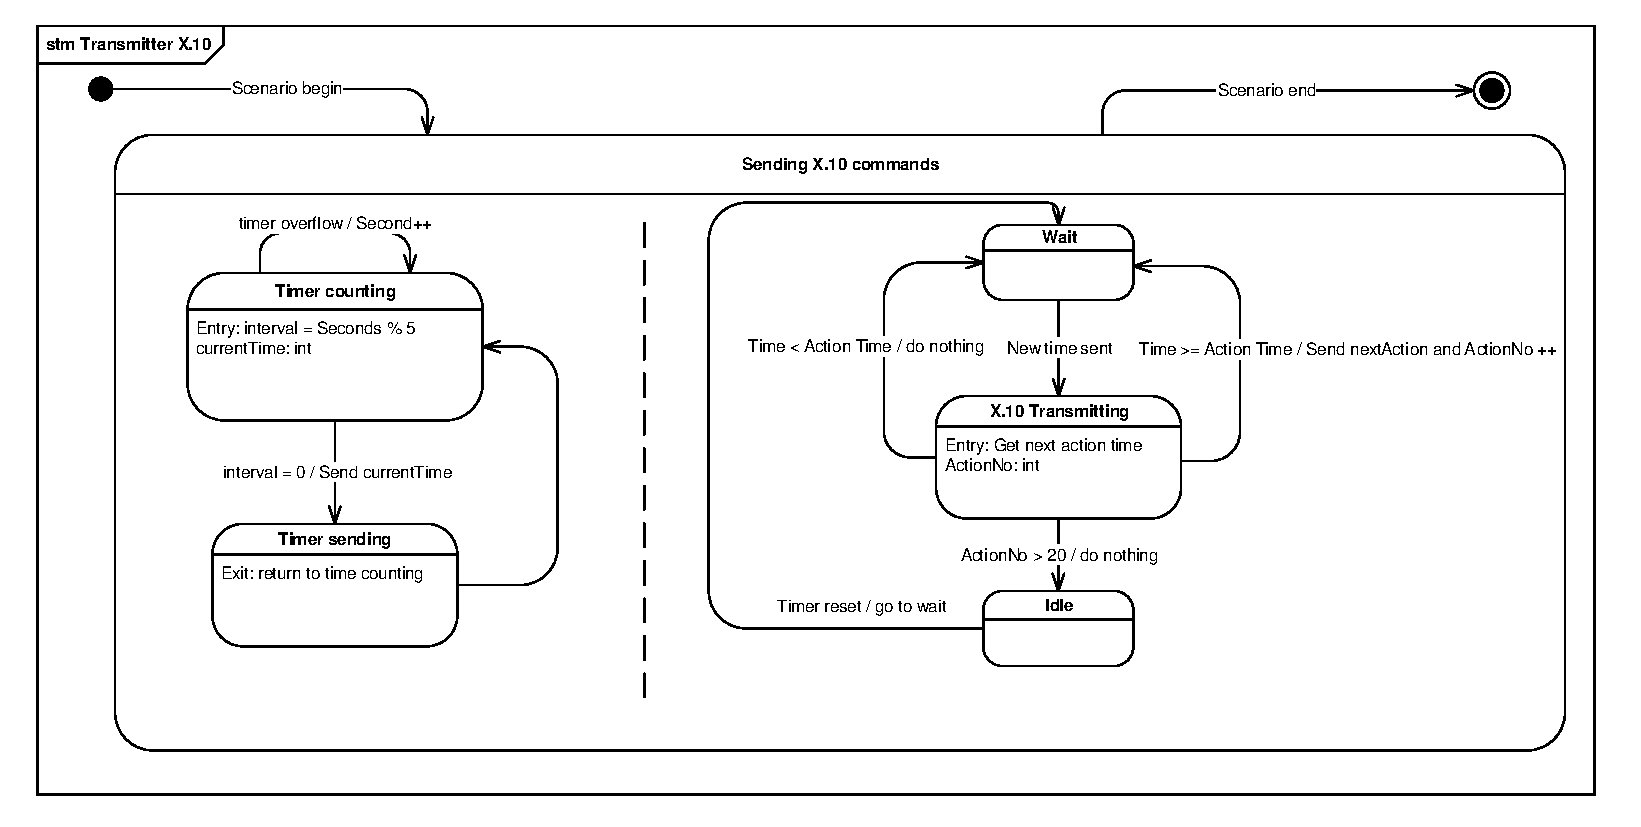
\includegraphics[width=\textheight + 190pt,clip=true, trim=18 15 18 12]{Systemarkitektur/diagrammer/Stm_transmitter_X10} %L B R T - HUSKE DET
\end{figure}

Denne statemachine viser det parallele forløb mellem Time, som holder styr på tiden, og transmitteren, der modtager tid fra Time, samt sender X.10 data ud til Tx10 Klassen.

\clearpage

\subsubsection{Statemachine over X.10/receiver}

\begin{figure}[h]
\centering
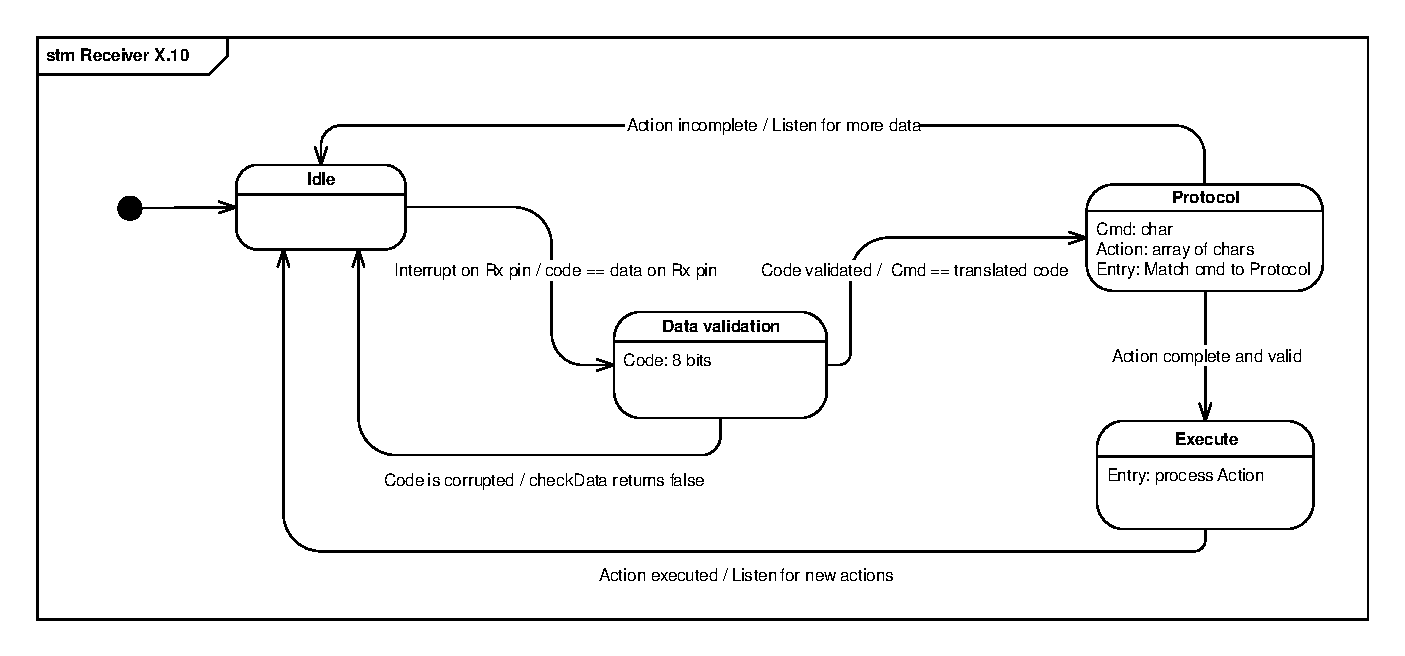
\includegraphics[width=\textheight + 190pt,clip=true, trim=18 15 15 12]{Systemarkitektur/diagrammer/Stm_receiver_X10}
\end{figure}

Her ses de forskellige tilstande receiveren skal gennemgå, når data modtages fra X.10 nettet. Når data modtages, loades de ind i en buffer, og checkes op mod X.10 protokollen. Hvis kommandoen er korrekt, vil den blive eksekveret, ellers skal den kastede kommandoen væk. Receiven lytter derefter for mere data. 



\end{landscape}

\clearpage